\chapter{Espacios vectoriales}

\lettrine[lines=7] {\initfamily \selectfont H} {emos} llegado a la parte central de esta tesis. En el capítulo anterior definimos y describimos las propiedades de los conjuntos de corte y las subgráficas pares de una gráfica $G$. El lector observador podrá haberse dado cuenta que la operación \textit{diferencia simétrica} $\triangle$ jugó un papel fundamental. En este capítulo estaremos dedicados a describir los diferentes espacios vectoriales asociados a las gráficas y digráficas. Posteriormente, estudiaremos sus relaciones con sus matrices de incidencia.

\section{Espacios en gráficas}
A menos que se mencione lo contrario, en esta sección supondremos que $G$ es una gráfica conexa con $n$ vértices y $m$ aristas, de tal manera que $V(G)=\{u_{1}, \ldots, u_{n}\}$ y $A(G) = \{e_{1}, \ldots, e_{m}\}$.

\subsection{Espacio de aristas $\mathcal{E}(G)$}
Denotaremos por $\mathcal{E}(G)$ al conjunto de subgráficas generadoras de $G$.
Es muy sencillo verificar que la operación $\triangle$ es cerrada en $\mathcal{E}(G)$. En efecto, dadas $F_{1}, F_{2} \in \mathcal{E}(G)$, se tiene que  $F_{1} \bigtriangleup F_{2} \in \mathcal{E}(G)$, pues $E(F_{1}) \triangle E(F_{2}) \subseteq E(G)$ y los vértices de $G$ se mantienen invariantes. Nótese que la subgráfica $\varnothing$ funciona como elemento neutro de $\triangle$.

Podemos también definir un producto interior en $\mathcal{E}(G)$ bajo el campo $GF(2)$. Dados $\lambda \in GF(2)$ y $H$ una subgráfica generadora de $G$, consideramos el producto escalar $\cdot$ dado por:
$$
\lambda \cdot H =\left\{\begin{matrix}
H, & \lambda = 1  \\
\varnothing, & \lambda = 0.
\end{matrix}\right.
$$

    \index{Espacio! de aristas}Debido a la naturaleza y propiedades de la diferencia simétrica $\triangle$, es muy fácil darse cuenta que la terna $\Big(\mathcal{E}(G), \triangle, \cdot\Big)$ es un espacio vectorial sobre el campo $GF(2)$. Es por esto que a $\mathcal{E}(G)$ se le conoce como el \textit{espacio de aristas de} $G$. 


Las subgráficas generadoras inducidas $G[\{e_{i}\}]$ (es decir, tomamos cada arista de $G$ como una subgráfica generadora) forman una base de $\mathcal{E}(G)$. En efecto, $\Big\{G[\{e_{i}\}]\Big|\:\! i = 1,\ldots, m\Big\}$ es un conjunto generador pues, para toda $H \in \mathcal{E}(G)$, $$H = \difsym_{e \in E(H)} G[\{e\}].$$ Además, es linealmente independiente debido a que $\lambda_{1}G[\{e_{1}\}] \triangle \cdots \triangle \lambda_{m}G[\{e_{m}\}] = \varnothing$ si y sólo si, para toda $i = 1, \ldots, m$, $\lambda_{i}=0$,porque $\varnothing$ no tiene aristas. Por lo tanto, $\Big\{G[\{e_{i}\}]\Big|\:\! i = 1,\ldots, m\Big\}$ es una base de $\mathcal{E}(G)$.

De lo anterior, concluimos que $\dim(\mathcal{E}(G)) = m$. Una consecuencia de conocer una base de $\mathcal{E}(G)$ y su dimensión es que podemos saber el número total de elementos en el espacio de aristas. Ya que nuestro campo $GF(2)$ es finito y consta de dos elementos (el $0$ y el $1$), tomar combinaciones lineales de la base es equivalente a tomar subconjuntos de ésta. 

¿Cuántos subconjuntos de $\Big\{G[\{e_{1}\}],\ldots, G[\{e_{m}\}]\Big\}$ hay? De la Combinatoria se sabe que existen $2^{m}$ subconjuntos de un conjunto de $m$ elementos. Así, sencillamente, deducimos que $|\mathcal{E}(G)| = 2^{m}$.

\begin{ejem}
 \begin{figure}[H]
 %\vspace{-0.5cm}
    \centering
    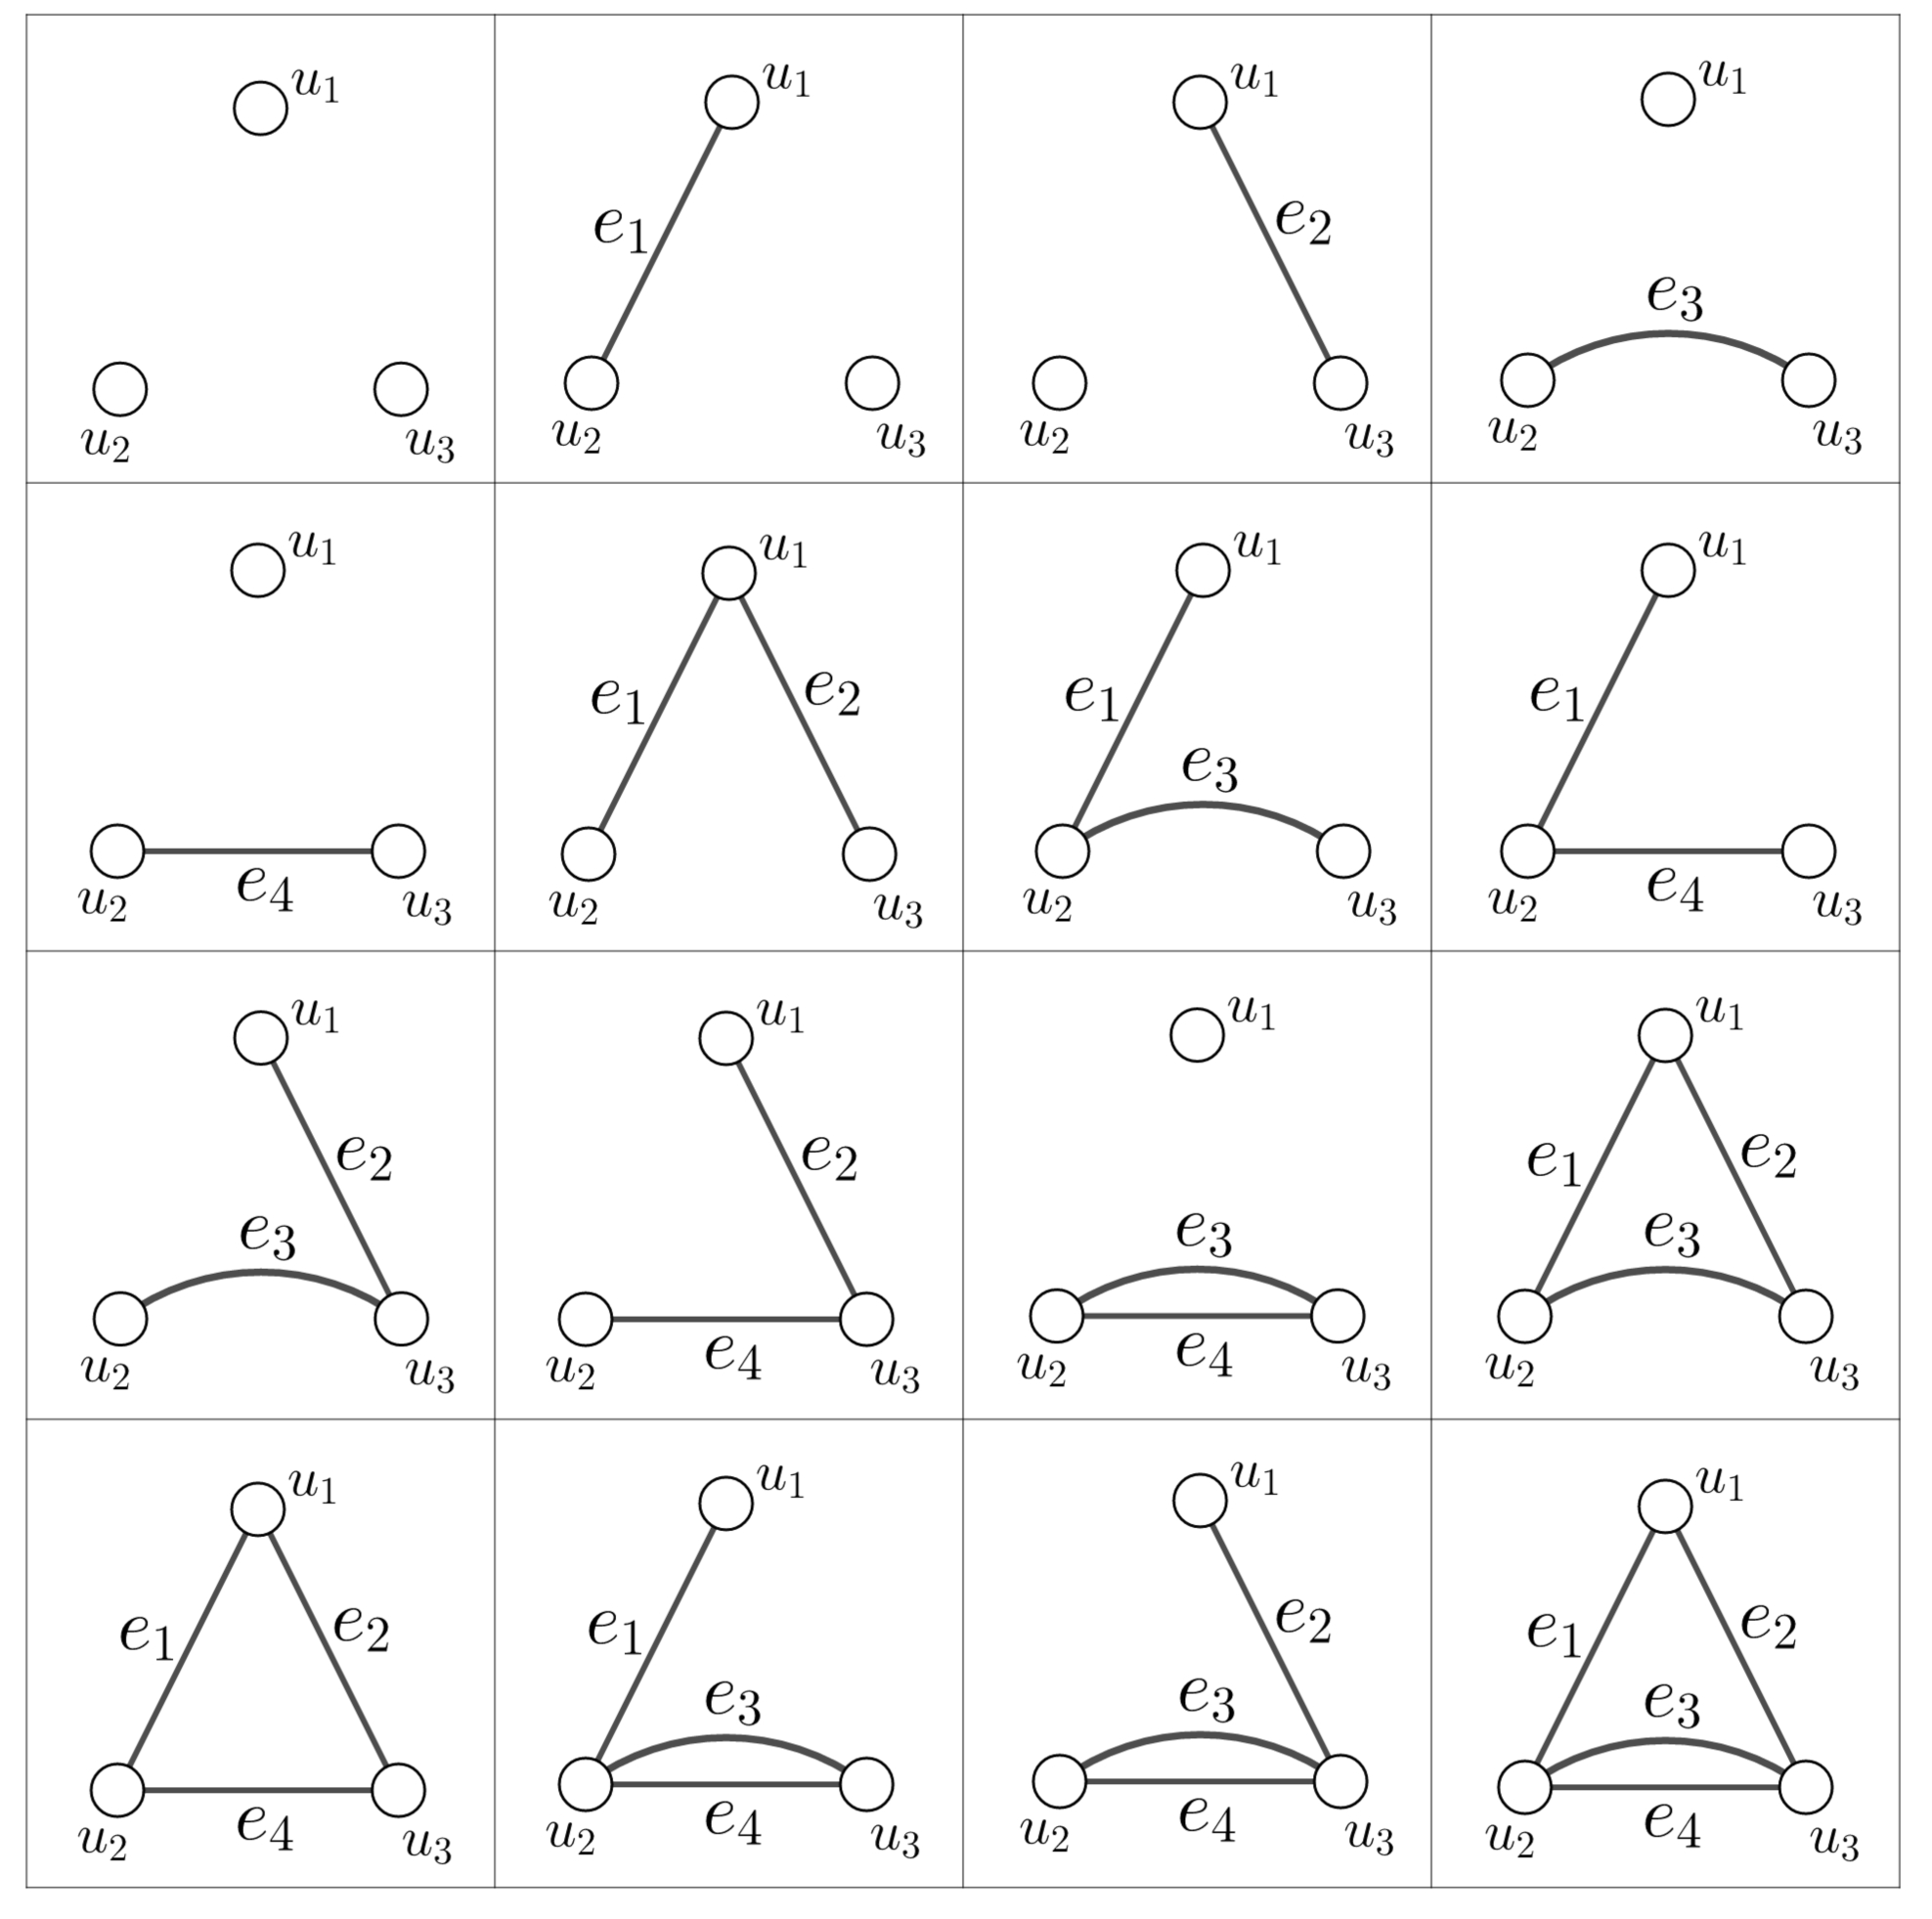
\includegraphics[scale=0.7]{img/imgchapter3/espacioaristas.jpg}
    %height=0.8\textheight
    %width=0.7\textwidth
    \caption{Espacio de aristas}
    \label{fig:edgespace}
\end{figure}
 
 \begin{figure}[H]
   %\vspace{-0.8cm}
    \centering
    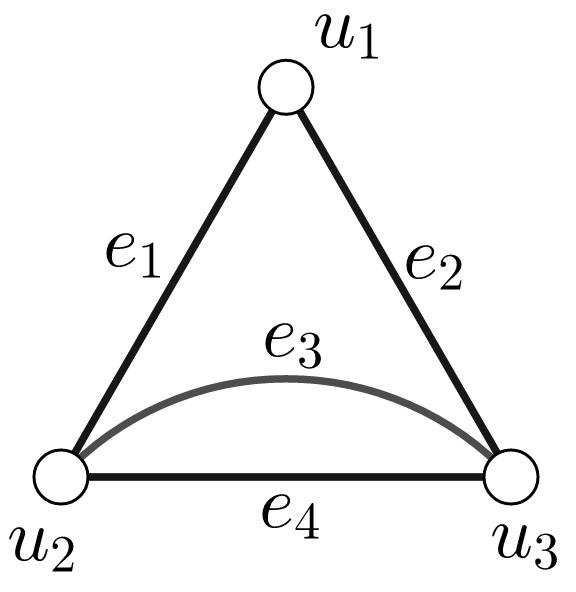
\includegraphics[scale=0.3]{img/imgchapter3/grafoejemplo.jpg}
    \caption{}
    \label{fig:grafoejemplo}
   % \vspace{-0.5cm}
\end{figure}

 Consideremos la gráfica de la figura \ref{fig:grafoejemplo}, la cual consta de cuatro aristas. En la imagen \ref{fig:edgespace} desglosamos su espacio de aristas. Nótese que hay $2^{4} = 16$ subgráficas generadoras.
 
 
\hfill $\blacklozenge$ 
\end{ejem}


\subsection{Espacio de conjunto de cortes $\mathcal{B}(G)$}
A la colección de las subgráficas generadoras inducidas por los conjuntos de corte de $G$ se  le denota por $\mathcal{B}(G)$. Así, $\mathcal{B}(G) \subseteq \mathcal{E}(G)$. De hecho, $\mathcal{B}(G)$ argumentaremos por qué éste resulta ser un subespacio vectorial de $\mathcal{E}(G)$.  

 \index{Espacio! de cortes}Si recordamos el corolario \ref{cor:difsimGeneradora}, su principal consecuencia es que \textit{la diferencia simétrica subgráficas generadoras inducidas por conjuntos de corte es también un conjunto de corte}, esto es, que $\mathcal{B}(G)$ es \textit{cerrado} bajo la diferencia simétrica $\triangle$: 

\begin{teo} \label{teo:difsimcortes}
\begin{center}
    Si $F_{1}, F_{2} \in \mathcal{B}(G)$, entonces $F_{1} \triangle F_{2} \in \mathcal{B}(G)$.
\end{center}
\end{teo}

Dado que $\varnothing$ es un corte y $\mathcal{B}(G)$ es trivialmente cerrado bajo el producto escalar, se sigue que \bond es un subespacio de $\mathcal{E}(G)$ y recibe el nombre de \textit{espacio de cortes de} $G$. En la figura \ref{fig:cortesw4} está desglosado el espacio de cortes de la gráfica $W_{4}$.

Asimismo, el corolario \ref{cor:unionajenademinimalesgeneradores} también puede formularse en términos propios del Álgebra Lineal:

\begin{teo}
\begin{center}
    Los conjuntos de corte minimales generan al subespacio \bondt.
\end{center}
\end{teo}


Además de los cortes minimales, existe otro conjunto de cortes que genera a $\mathcal{B}(G)$ y que nos será de mucha ayuda más adelante. Observemos que cualquier $X \subseteq V(G)$ puede expresarse como diferencia simétrica de sus elementos, es decir, $X = \difsym_{u \in X} \{u\}$. Por tanto, debido al corolario \ref{cor:cortessimInd}, el conjunto de corte asociado a $X$ puede expresarse así:
$$
\partial(X) = \difsym_{u \in X} \partial(\{u\}).
$$
Lo anterior da lugar al siguiente resultado:

\begin{prop} \label{prop:incidenceset}
La colección de subgráficas generadoras inducidas por los cortes de la forma $\partial(u)$, con $u \in V(G)$, es un conjunto generador del subespacio \bondt.
\end{prop}

Ya hemos construido conjuntos generadores. ¿Qué conjunto de cortes resulta ser una base para el espacio $\mathcal{B}(G)$? Traigamos a la memoria los cortes fundamentales de $G$. 

Dado $T$ un árbol generador de $G$, el teorema \ref{teo:basecortesfundamentales} implica que las subgráficas generadoras inducidas por los cortes fundamentales de $G$ determinan un conjunto generador. Aún más, afirmamos que son linealmente independientes. Tomemos una combinación lineal cualquiera de $\varnothing$, es decir, supongamos que  
$$
\difsym_{b \in E(T)} \lambda_{b}G[\mathscr{B}_{b}] = \varnothing,
$$
con $\lambda_{b} \in GF(2)$. Tomando $S\subseteq T$ con $E(S):=\{b \in E(T) | \:\! \lambda_{b} \neq 0\}$, tenemos
$$
\difsym_{b \in E(T)} \lambda_{b}G[\mathscr{B}_{b}] = \difsym_{b \in E(S)} \lambda_{b}G[\mathscr{B}_{b}]= \varnothing.
$$
Por el lema \ref{cortesfundamentalespropchida},  $\emptyset$ es el único corte tal que $\varnothing \cap E(T) = E(S)$. Luego, $E(S) = \emptyset$ y, en consecuencia, $\lambda_{b}=0$, para toda $b\in E(T)$. Por consiguiente, $\Big \{G[\mathscr{B}_{b}] \in \mathcal{B}(G) \Big|\: b\in E(T)\Big\}$ es un conjunto linealmente independiente. Ya que este mismo conjunto es generador,  necesariamente es una base. Tal hecho lo dejamos plasmado como un teorema.


\begin{teo}
La colección de las subgráficas generadoras inducias por los conjuntos de corte fundamentales respecto a un árbol $T$ es una base para \bondt.
\end{teo}

Sabemos que hay $n-1$ cortes fundamentales asociados a algún árbol generador de $G$, así que el teorema anterior nos permite deducir que $\dim(\mathcal{B}(G))=n-1$.

¿Qué sucede si $G$ no es conexa? Supongamos que $G = \bigcup_{j=1}^{c}F_{j}$ (esta unión es ajena), con $F_{1}, \ldots, F_{c}$ sus componentes conexas. Para cada $i \in \{1,\ldots, c\}$, definimos $\mathcal{F}_{i}$ como la subgráfica generadora de $G$ inducida por las aristas de $F_{i}$, es decir, $$\mathcal{F}_{i}:=G\Big[E(F_{i})\Big].$$

Entonces $G = \bigcup_{j=1}^{c}\mathcal{F}_{i}$ (esta unión sólo es ajena por aristas). Con base en los razonamientos que hicimos en el capítulo pasado, ya sabemos que toda subgráfica generadora inducida por un  corte de $\mathcal{F}_{j}$ es una subgráfica generadora inducida por un corte de $G$. Por lo que $\mathcal{B}(\mathcal{F}_{j}) \subseteq \mathcal{B}(G)$. Las subgráficas generadoras inducidas por cortes en $\mathcal{B}(\mathcal{F}_{j})$ corresponden a las subgráficas generadoras inducidas por los cortes en $\mathcal{B}(F_{j})$. Luego, $\dim(\mathcal{B}(\mathcal{F}_{j})) = \dim(\mathcal{B}(F_{j})) = |V(F_{j})| - 1$.

Además, todo subgráfica generadora inducida por corte de $G$ es una diferencia simétrica de subgráficas generadoras inducidas por cortes de cada subgráfica $\mathcal{F}_{j}$; y también es sencillo ver que $\varnothing$ es la única subgráfica generadora inducida por un conjunto de corte que tienen en común las subgráficas $\mathcal{F}_{i}$. 

Las ideas anteriores nos permiten asegurar que $\mathcal{B}(G)$ es suma directa de los subespacios $\mathcal{B}(\mathcal{F}_{j})$ (correspondientes a sus componentes conexas), es decir, $\mathcal{B}(G)= \mathcal{B}(\mathcal{F}_{1}) \oplus \cdots \oplus \mathcal{B}(\mathcal{F}_{c})$.

Luego entonces, 
\begin{align*}
    \dim(\mathcal{B}(G)) &= \sum_{j = 1}^{c}\dim(\mathcal{B}(\mathcal{F}_{j}))\\
    &= \sum_{j = 1}^{c} (|V(F_{j})| - 1) \\
    &= \sum_{j=1}^{c} |V(F_{j})| - \sum_{j=1}^{c} 1\\
    &= n - c.
\end{align*}

Concluimos, finalmente, con un teorema:

\begin{teo} \label{teo:dimcortes}
En toda gráfica $G$, la dimensión de su espacio de cortes $\mathcal{B}(G)$ es $n-c(G)$. Aún más, la cantidad de conjuntos de corte en dicho espacio es $2^{n-c(G)}$.
\end{teo}

\subsection{Espacio de ciclos $\mathcal{C}(G)$}

El conjunto $\mathcal{C}(G) \subseteq \mathcal{E}(G)$ es la colección de las subgráficas generadoras pares y es el segundo subespacio vectorial de $\mathcal{E}(G)$ a considerar.

El teorema \ref{teo:difsimciclos}  implica que $\mathcal{C}(G)$ es cerrado bajo diferencias simétricas. Como $\varnothing$ es una subgráfica par y $\mathcal{C}(G)$ es trivialmente cerrado bajo el producto escalar, tenemos que $\mathcal{C}(G)$ es un subespacio de $\mathcal{E}(G)$ y recibe el nombre de \index{Espacio! de ciclos} \textit{espacio de ciclos de} $G$. En la figura \ref{fig:espaciociclos} está desglosado el espacio de ciclos de $W_{4}$.

\begin{teo} \label{teo:difsimciclos2}
La diferencia simétrica de dos subgráficas pares es, a su vez, una subgráfica par, es decir, si $C_{1},C_{2} \in$ \cyclet, entonces $C_{1} \triangle C_{2}\in$ \cyclet
\end{teo}

Por otro lado, el corolario \ref{teo:veblen2} proporciona un conjunto generador para el espacio de ciclos:

\begin{teo}
\begin{center}
    La colección de ciclos de $G$ genera al subespacio \cyclet.
\end{center}
\end{teo}

Como el lector seguramente estará pensando, basándonos en el teorema \ref{cor:baseciclosfundamentales}, la colección de ciclos fundamentales es una base de $\mathcal{C}(G)$ y lo probamos en seguida.

\begin{teo}
El conjunto de ciclos fundamentales respecto a un árbol generador $T$ es una base para \cyclet.
 \end{teo}
 
 \begin{proof} Sean $T$ un árbol generador de $G$ y $\{\mathscr{C}_{c} \in \mathcal{C}(G) | c \in E(\overline{T})\}$ el conjunto de sus respectivos ciclos fundamentales. El corolario \ref{cor:baseciclosfundamentales} implica que los ciclos fundamentales respecto a $T$ conforman un conjunto generador de $\mathcal{C}(G)$. Veamos ahora que dicho conjunto es linealmente independiente.
 
Supongamos que $$\difsym_{c \in E(\overline{T})} \lambda_{c}\mathscr{C}_{c} = \varnothing,$$ con $\lambda_{c} \in GF(2)$.  Tomando $S\subseteq \overline{T}$ con $E(S):=\{c \in E(\overline{T}) | \lambda_{c} \neq 0\}$, tenemos
$$
\difsym_{c \in E(\overline{T})} \lambda_{c}\mathscr{C}_{c} = \difsym_{c \in E(S)} \lambda_{c}\mathscr{C}_{c}= \varnothing.
$$
Por la proposición \ref{ciclosfundamentalespropchida},  $\varnothing$ es la única subgráfica tal que $\varnothing \cap \overline{T} = S$. Luego, $S = \varnothing$ y, en consecuencia, $\lambda_{c}=0$, para toda $c \in E(\overline{T})$. Por consiguiente, $\{\mathscr{C}_{c} \in \mathcal{C}(G) | c \in E(\overline{T})\}$ es un conjunto linealmente independiente. 

Al ser linealmente independiente y generador, el conjunto de ciclos fundamentales es una base de $\mathcal{C}(G)$

 \end{proof}

Sabemos que hay $m -n+1$ ciclos fundamentales asociados a algún árbol generador de $G$, así que el teorema anterior nos permite deducir que $\dim(\mathcal{C}(G))=m-n+1$.

¿Qué sucede si $G$ no es conexa? Suponiendo que $G = \bigcup_{j=1}^{c}F_{j}$, con $F_{1}, \ldots, F_{c}$ sus componentes conexas; los mismos razonamientos que hicimos antes nos permiten considerar al subespacio \\$\mathcal{C}(\mathcal{F}_{j}) \subseteq \mathcal{C}(G)$. Ya que $\varnothing$ es la única subgráfica generadora par que tienen en común los subespacios $\mathcal{C}(\mathcal{F}_{j})$ y que toda gráfica par es unión ajena de ciclos, entonces $\mathcal{C}(G)$ de los subespacios $\mathcal{C}(\mathcal{F}_{j})$, es decir, $$\mathcal{C}(G)= \mathcal{C}(\mathcal{F}_{1}) \oplus \cdots \oplus \mathcal{C}(\mathcal{F}_{c}).$$

Como lo elementos de $\mathcal{C}(\mathcal{F}_{j})$ corresponden a los de $\mathcal{C}(F_{j})$, entonces $$\dim(\mathcal{C}(\mathcal{F}_{j})) = \dim(\mathcal{C}(F_{j})) = |E(F_{j})|-|V(F_{j})| + 1.$$

Luego entonces, 
\begin{align*}
    \dim(\mathcal{C}(G)) &= \sum_{j = 1}^{c}\dim(\mathcal{C}(\mathcal{F}_{j}))\\
    &= \sum_{j = 1}^{c} (|E(F_{j})|-|V(F_{j})| + 1) \\
    &= \sum_{j=1}^{c} |E(F_{j})| - \sum_{j=1}^{c} |V(F_{j})| + \sum_{j=1}^{c} 1\\
    &= m - n + c.
\end{align*}

Concluyendo así con el siguiente resultado.

\begin{teo}\label{teo:dimciclos}
En toda gráfica $G$, la dimensión de su espacio de ciclos $\mathcal{C}(G)$ es $m -n +c(G)$. Aún más, la cantidad de gráficas pares en dicho espacio es $2^{m-n+c(G)}$.
\end{teo}


\section{Vectores de incidencia}

En el capítulo $1$ comentamos que si $V$ es un espacio vectorial sobre un campo $\mathbb{F}$ de dimensión $n$, entonces $V$ es isomorfo al espacio $\mathbb{F}^n$. Ahora aplicaremos esta idea a los espacios que hemos definido en las secciones anteriores.

Sabemos que el espacio de aristas $\mathcal{E}(G)$ es de dimensión $m$ sobre el campo $GF(2)$. Se sigue entonces que $\mathcal{E}(G)$ es isomorfo a $(GF(2))^{m}$. 

Una forma inmediata de identificar a $\mathcal{E}(G)$ con $(GF(2))^{m}$ se describe a continuación. Tomando $H \in \mathcal{E}(G)$, la \textit{función de incidencia de} $H$ es la función característica de $E(H)$, $$\chi_{H} := \chi_{E(H)} : E(G) \rightarrow GF(2),$$ dada por:

 $$
 \chi_{H}(e) = \left\{\begin{matrix}
1, & \text{si} \hspace{1.5mm} e \in E(H) \\ 
0, & \text{si} \hspace{1.5mm} e\notin E(H).
\end{matrix}\right.
 $$
 
 \index{Vector! de incidencia} Como el conjunto de aristas de $G$ ya está ordenado, es decir, que $E(G) = \{e_{1}, \ldots, e_{m}\}$, las funciones de incidencia pueden escribirse como vectores. En efecto, dada $H \in \mathcal{E}(G)$, identificamos la función de incidencia de $H$, con el vector $\boldsymbol{\chi}_{H}^{\textnormal{T}}:= (\chi_{H}(e_{1}), \ldots, \chi_{H}(e_{m})) \in (GF(2))^{m}$ y lo llamamos \textit{vector de incidencia de} $H$.
 
 Podemos definir ahora una función que hace corresponder cada subgráfica generadora con su respectivo vector de incidencia, a saber, la función $\boldsymbol{\Phi} \colon \mathcal{E}(G) \rightarrow (GF(2))^{m}$ tal que, para cada $H \in \mathcal{E}(G)$, $\boldsymbol{\Phi}(H) = \boldsymbol{\chi}_{H}$. Entonces $\boldsymbol{\Phi}$ es un isomorfismo entre $\mathcal{E}(G)$ y el espacio $(GF(2))^{m}$.
 En la imagen \ref{fig:grafovector1} mostramos (de forma simbólica) los vectores de incidencia de algunas subgráficas de la gráfica de la figura \ref{fig:grafoejemplo}.

 \begin{figure}[H]
    \centering
    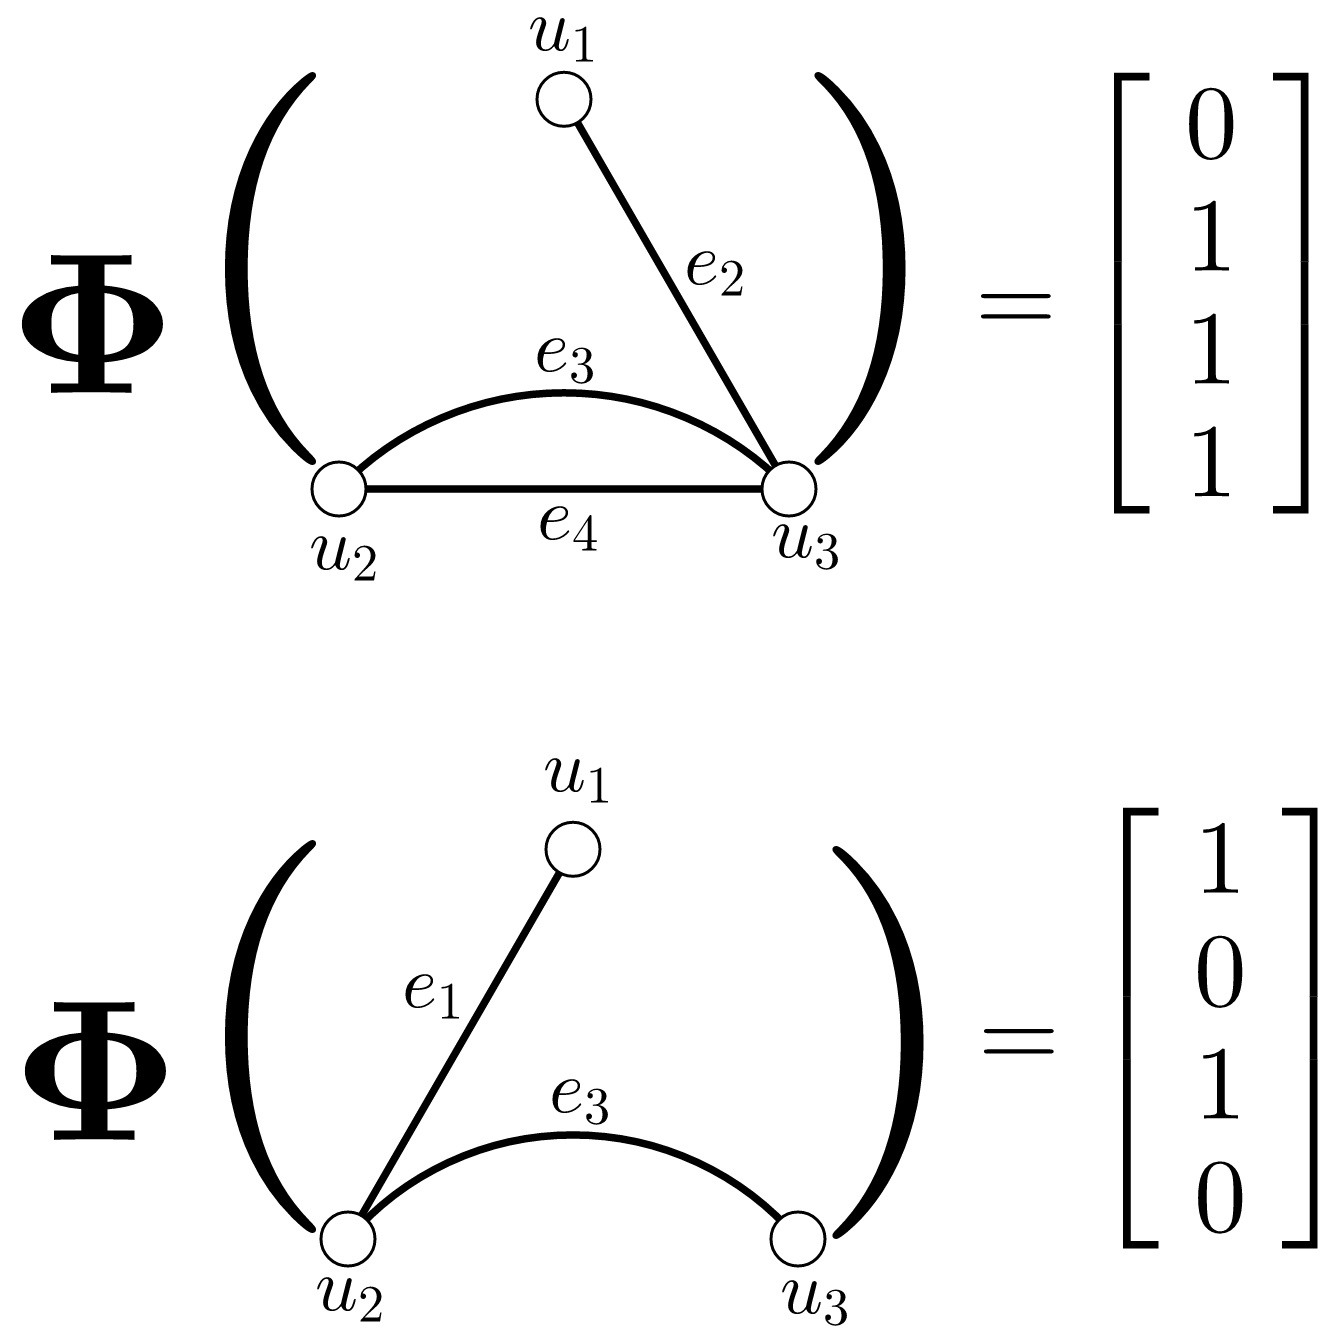
\includegraphics[scale=0.2]{img/imgchapter3/grafovector1.jpg}
    \caption{}
    \label{fig:grafovector1}
    %\vspace{-0.5cm}
\end{figure}


Como el isomorfismo $\boldsymbol{\Phi}$ preserva las operaciones entre los espacios vectoriales correspondientes, la diferencia simétrica $\triangle$ en $\mathcal{E}(G)$ es equivalente a la operación $\oplus$ en $(GF(2))^{m}$ (que describimos en el capítulo $1$), es decir, $$\boldsymbol{\Phi}(H_{1} \triangle H_{2}) = \boldsymbol{\Phi}(H_{1}) \oplus \boldsymbol{\Phi}(H_{2}).$$ La conclusión más importante de esta discusión es que cada subgráfica de $G$ ``se codifica'' en un vector binario. Todo vector de ceros y unos puede ``traducirse'' en una subgráfica generadora de $G$, cuyas aristas corresponderán a las entradas del vector que son iguales a $1$. El siguiente teorema resume lo dicho hasta aquí.


\begin{teo} \label{teo:xor}
Sea $G$ una gráfica cualquiera. Para cualesquiera $H_{1}, H_{2} \in \mathcal{E}(G)$, se cumple que $$\boldsymbol{\chi}_{H_{1} \triangle H_{2}} = \boldsymbol{\chi}_{H_1} \oplus \boldsymbol{\chi}_{H_2}.$$
\end{teo}

\begin{ejem}
Ilustramos lo comentado líneas arriba considerando de nuevo la gráfica $G$ de la figura \ref{fig:grafoejemplo}. En esta ocasión, en la imagen \ref{fig:operacionesisomorfismo} aplicamos la operación $\triangle$ a las dos subgráficas de la figura \ref{fig:grafovector1} y también sumamos sus respectivos vectores de incidencia. Puede notarse que la diferencia simétrica en $\mathcal{E}(G)$ es equivalente a la operación $\oplus$ en $(GF(2))^{m}$. 

\begin{figure}[H]
    \centering
    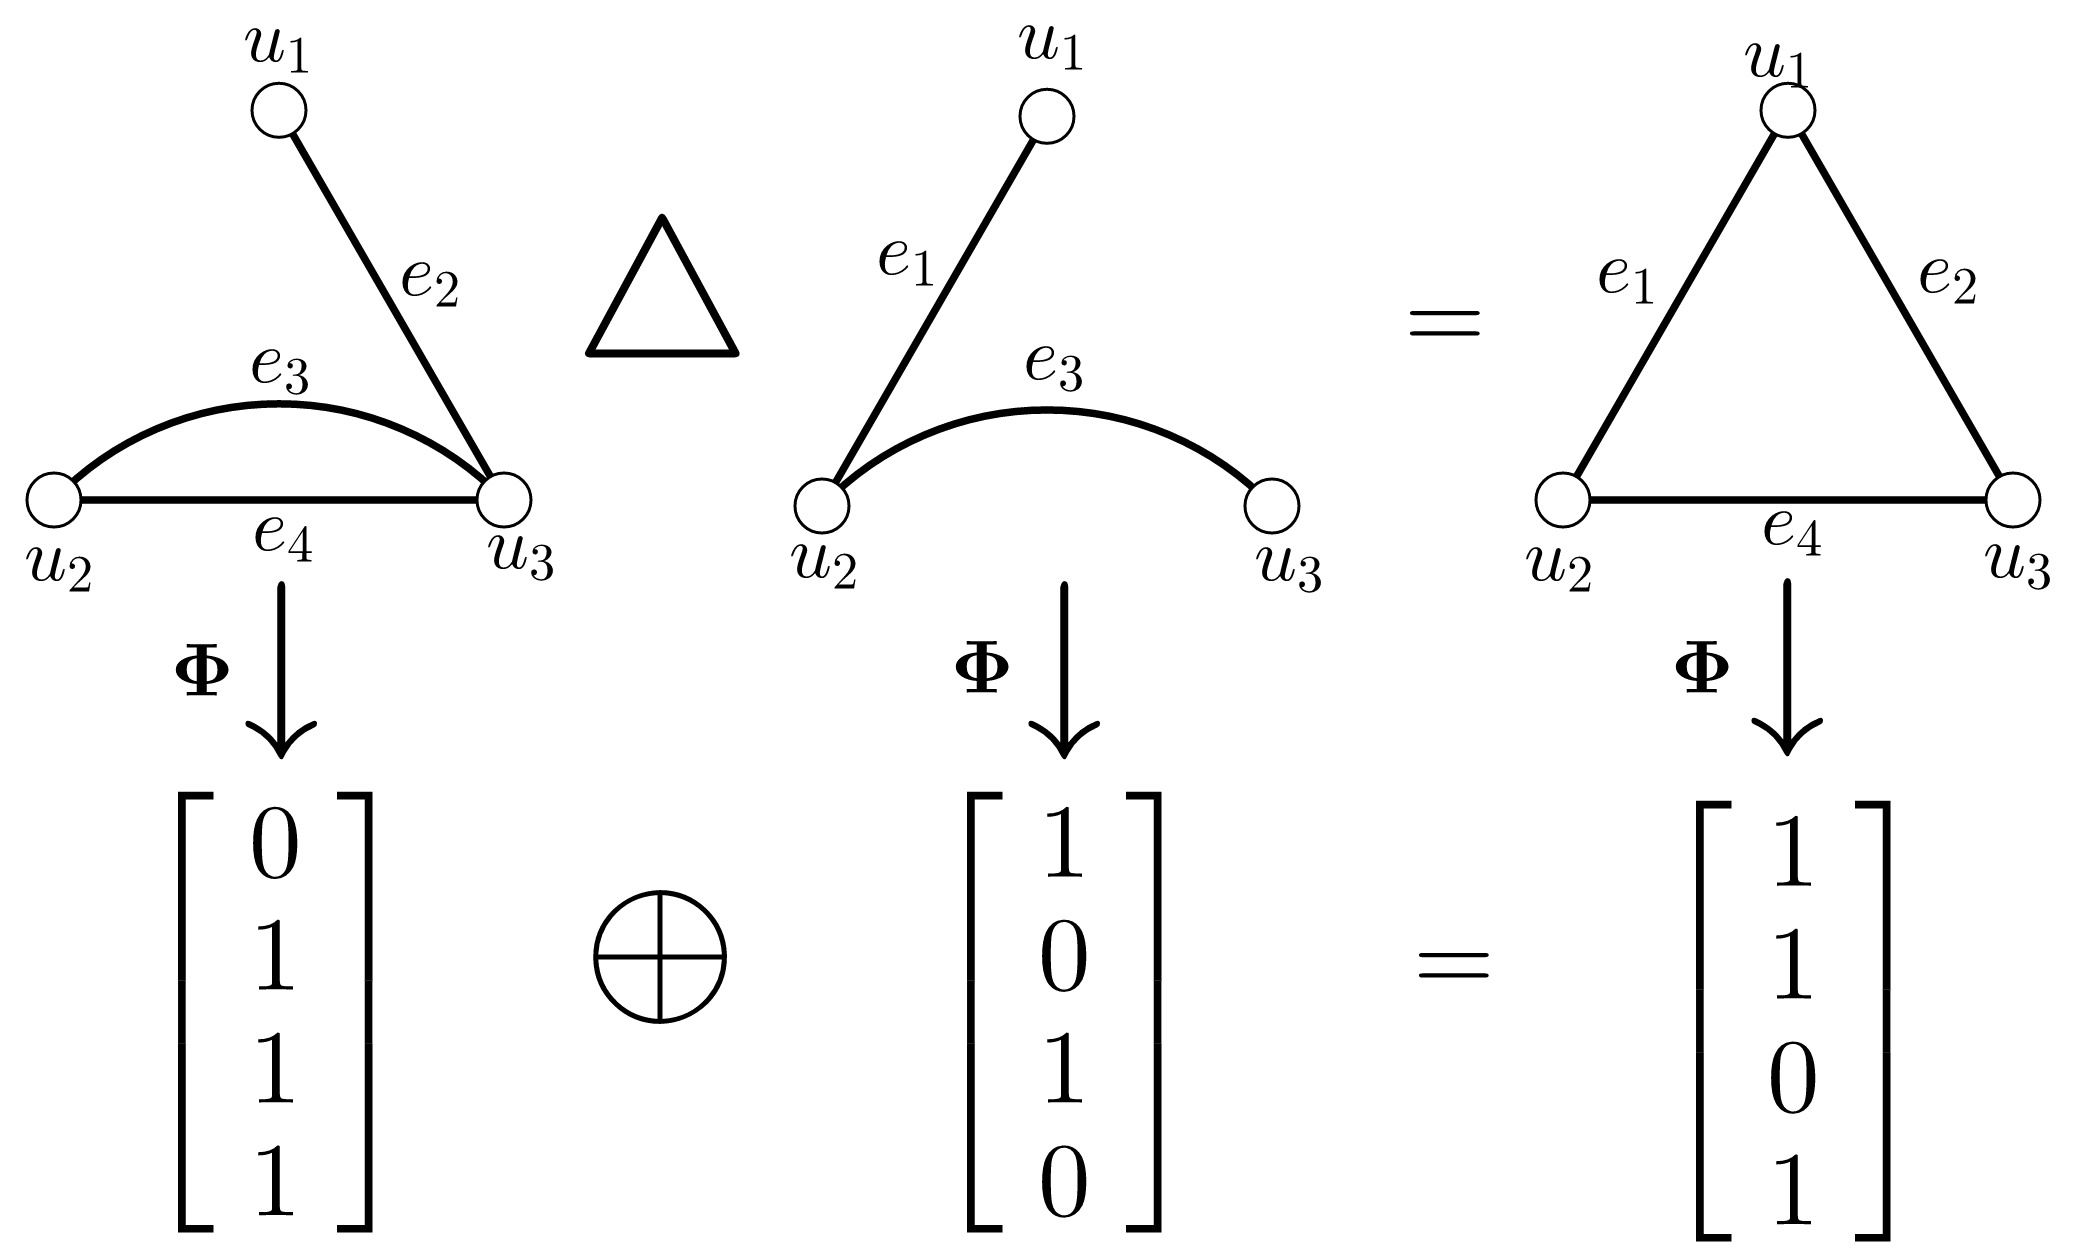
\includegraphics[scale=0.2]{img/imgchapter3/operacionesisomorfismo.jpg}
    \caption{}
    \label{fig:operacionesisomorfismo}
\end{figure}

\hfill $\blacklozenge$
\end{ejem}

Naturalmente, los conjuntos de corte y las subgráficas pares también se \textit{traducen} en vectores binarios. Los espacios $\overrightarrow{\mathcal{E}}(G):=\boldsymbol{\Phi}[\mathcal{E}(G)]$, $\overrightarrow{\mathcal{B}}(G):=\boldsymbol{\Phi}[\mathcal{B}(G)]$ y $\overrightarrow{\mathcal{C}}(G):=\boldsymbol{\Phi}[\mathcal{C}(G)]$ son conocidos también como \textit{los espacios de aristas, de cortes} y \textit{de ciclos en sí}, respectivamente (aunque, formalmente, es un abuso de la nomenclatura que utilizamos en esta tesis). Note que $\overrightarrow{\mathcal{B}}(G)$ es isomorfo a $(GF(2))^{n-c(G)}$ y a $\mathcal{B}(G)$; mientras que $\overrightarrow{\mathcal{C}}(G)$ es isomorfo a $(GF(2))^{m-n+c(G)}$ $\mathcal{C}(G)$.

Una ventaja que nos proporcionan los vectores de incidencia es la posibilidad de definir un producto interior en $\mathcal{E}(G)$, utilizando el ya existente en $(GF(2))^{m}$. Así, dadas $H$ y $F$ subgráficas generadoras cualesquiera de $G$, definimos el \textit{producto interior de} $H$ \textit{y} $F$ como:

$$
\langle H,F \rangle  :=  \langle \boldsymbol{\chi}_{H},\boldsymbol{\chi}_{F}\rangle =  \sum_{i=1}^{m} \chi_{H}(e_{i}) \cdot \chi_{F}(e_{i}) \quad \text{(mod }2).
$$

Cabe recordar que este producto interno es \textit{degenerado} pues, claramente, si una subgráfica $H \neq \varnothing$ tiene una cantidad par de aristas, entonces $\langle H,H\rangle = 0$.

Respecto a la paridad, ésta nos brinda una noción de \textit{ortogonalidad}. Recordando el teorema \ref{teo:interseccionpar}, sabemos que todo elemento de $\mathcal{B}(G)$ y $\mathcal{C}(G)$ coinciden en un número par de aristas. Esto, a la luz de nuestro nuevo producto interno, puede reescribirse así:

\begin{teo}
Todo conjunto de corte de $G$ es ortogonal a cualquier subgráfica par de $G$.
\end{teo}


Gracias a los conceptos de álgebra lineal desglosados en el primer capítulo, y con apoyo de este último teorema, concluimos que \bond y \cycle son complementos ortogonales. Es decir:

$$
\mathcal{B}(G)=(\mathcal{C}(G))^{\perp} \quad \text{y} \quad \mathcal{C}(G)=(\mathcal{B}(G))^{\perp}. 
$$

Sin embargo, a pesar de ser complementos ortogonales, no siempre sucede que $\mathcal{E}(G) = \mathcal{B}(G) \oplus \mathcal{C}(G)$, pues hay gráficas que tienen subgráficas no vacías que son, al mismo tiempo, conjuntos de corte y gráficas pares (subgráficas ortogonales consigo mismas); en otras palabras, existen gráficas tales que $\mathcal{B}(G) \cap \mathcal{C}(G) \neq \{ \varnothing\}$. Vimos en el ejemplo \ref{ejem:k4ciclocorte} que $K_{4}$ es una gráfica con tales características.

\section{La matriz de incidencia de $G$}
Cuando se introdujo la matriz de incidencia en el capítulo $1$, se hizo considerando sus entradas en el campo de los número reales $\mathbb{R}$.

No obstante, si tomamos $\mathbf{M}:=\mathbf{M}_{G}$ en $M_{n \times m}(GF(2))$ surgen propiedades bastante interesantes que se relacionan con los espacios vectoriales que hemos estudiado a lo largo de este capítulo. En esta sección cada vez que mencionemos a la matriz de incidencia, lo haremos pensando que sus entradas están en $GF(2)$. Igualmente, recordemos que los vértices y las aristas de $G$ ya están ordenados, es decir, que $V(G)=\{u_{1}, \ldots, u_{n}\}$ y $E(G) = \{e_{1}, \ldots, e_{m}\}$

Una primera observación tiene que ver con lo que sucede si una gráfica tiene lazos. Cuando $\mathbf{M} \in M_{n \times m}(\mathbb{R})$, recordemos que se colocaba un ``$2$'' en la entrada del renglón y la columna que corresponden al vértice y al lazo respectivamente. Al cambiar de campo, ese ``$2$'' se vuelve un ``$0$''. Entonces las columnas de $\mathbf{M}$ que representan los lazos de $G$  son columnas cuyas entradas son todas cero.

\begin{ejem}
En la figura \ref{matrizdeincidenciagf2} mostramos la matriz de incidencia (¡pero en $GF(2)$!) de la misma gráfica de la imagen \ref{fig:matrizdeincidencia}.
\begin{figure}[H]
    \centering
    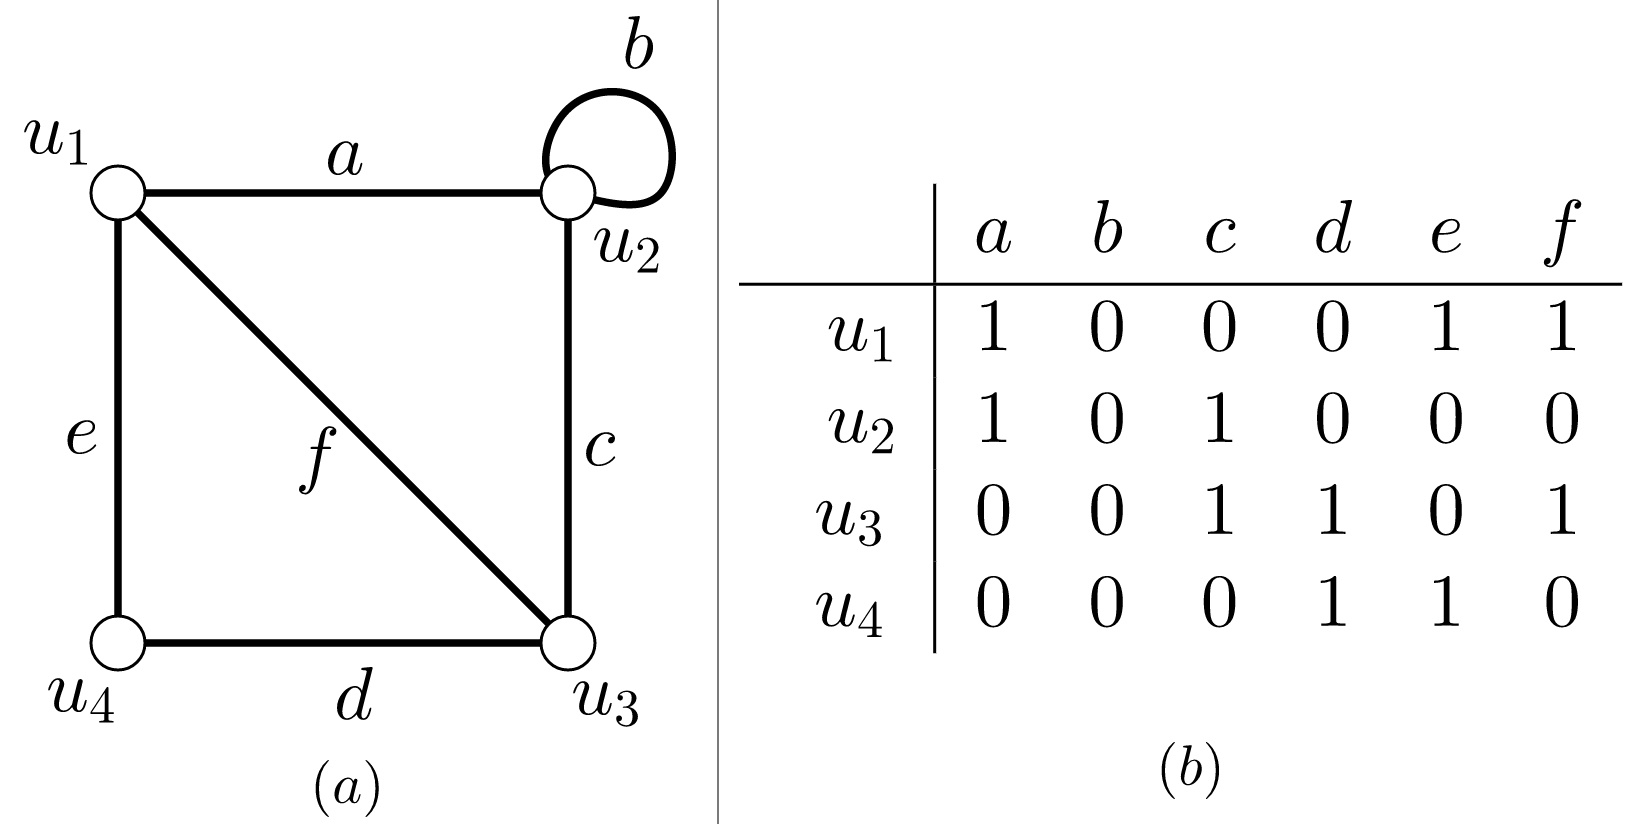
\includegraphics[scale=0.25]{img/imgchapter3/matrizdeincidenciagf2.jpg}
    \caption{}
    \label{matrizdeincidenciagf2}
\end{figure}
\vspace{-0.5cm}
\hfill $\blacklozenge$
\end{ejem}


Para simplificar nuestra notación, si $B$ es un conjunto de corte de $G$, entonces denotamos por $\boldsymbol{\chi}_{B}$ al vector de incidencia de $G[B]$, la subgráfica generadora inducida por $B$; y diremos, simplemente, que $\boldsymbol{\chi}_{B}$ es el \textit{vector de incidencia del conjunto de corte $B$}. En otro términos:
$$\boldsymbol{\chi}_{B}:= \boldsymbol{\chi}_{G[B]}.$$

Por otro lado, es fácil notar que cada renglón de $\mathbf{M}$ es el vector de incidencia del conjunto de corte asociado al vértice correspondiente a dicho renglón. Es decir:
$$\mathbf{M} = 
\begin{bmatrix}
\boldsymbol{\chi}_{\partial(u_{1})}^{\mathbf{t}}\\ 
\-- \\
\vdots \\
\-- \\
\boldsymbol{\chi}_{\partial(u_{n})}^{\mathbf{t}} 
\end{bmatrix}.
$$

En virtud de la proposición \ref{prop:incidenceset}, junto con el teorema \ref{teo:xor}, deducimos que:
$$
\mathsf{R}(\mathbf{M}) = span(\{ \boldsymbol{\chi}_{\partial(u_{1})}, \ldots, \boldsymbol{\chi}_{\partial(u_{n})} \}) = \overrightarrow{\mathcal{B}}(G).
$$

Esta igualdad la establecemos en el siguiente teorema.

\begin{teo}
\begin{center}
    El espacio generado por los renglones de $\mathbf{M}$ es $\overrightarrow{\mathcal{B}}(G)$.
\end{center}
\end{teo}

Ya sabemos que $Ker(\mathbf{M}) = (\textsf{R}(\mathbf{M}))^{\perp}$. Pero $\textsf{R}(\mathbf{M}))^{\perp} = (\overrightarrow{\mathcal{B}}(G))^{\perp}$ y, además, $\overrightarrow{\mathcal{C}}(G)=(\overrightarrow{\mathcal{B}}(G))^{\perp}$. Entonces $Ker(\mathbf{M}) =\overrightarrow{\mathcal{C}}(G) $. Tenemos, pues, el corolario siguiente. 

\begin{cor}
\begin{center}
    El espacio nulo de $\mathbf{M}$ es $\overrightarrow{\mathcal{C}}(G)$.
\end{center}
\end{cor}

\subsection{Rango y nulidad de $\mathbf{M}_{G}$}

Con la información obtenida de estas últimas proposiciones ya podemos conocer el rango de $\mathbf{M}$ y su nulidad. Gracias al capítulo $1$, se sabe que el rango de la matriz de incidencia es la dimensión del espacio generado por los renglones (o columnas también), es decir, $rank(\mathbf{M}) = \dim(\mathsf{R}(\mathbf{M}))$. Pero el espacio generado por los renglones es el espacio de cortes, cuya dimensión es $n-c$ (por el teorema \ref{teo:dimcortes}). Luego, haciendo $c:=c(G)$, $$rank(\mathbf{M}) = \dim(\mathsf{R}(\mathbf{M})) = \dim(\mathcal{B}(G)) = n - c.$$  Asimismo, con base en el teorema \ref{teo:dimciclos}, podemos deducir que $$null(\mathbf{M})=\dim(Ker(\mathbf{M}))= \dim(\mathcal{C}(G)) = m - n + c.$$ Obtenemos así lo siguiente.

\begin{teo} 
En $GF(2)$
se cumple que el rango de $\mathbf{M}$ es $n-c$ y su nulidad es $m -n +c$.
\end{teo}

\index{Rango! de una gráfica} \index{Nulidad! de una gráfica} Definimos el \textit{rango de $G$} como el número $\rho(G) :=  rank(\mathbf{M}) = n -c$ y la \textit{nulidad de $G$} como $\mu(G):= null(\mathbf{M}) = m - n + c$.

\subsection{Matrices reducidas}

Otra característica relevante de $\mathbf{M}$ es que la suma de todos sus renglones es igual al vector $\mathbf{0}$. En efecto, por el teorema \ref{teo:xor}, tenemos:
$$
\bigoplus_{i=1}^{n} \boldsymbol{\chi}_{\partial(u_{i})} = \boldsymbol{\chi}_{\partial(V(G))} = \boldsymbol{\chi}_{\varnothing} = \mathbf{0}.
$$

También uno podría darse cuenta de esto notando que como sólo hay dos ``1'' en cada columna (o ninguno si la arista asociada  a la columna es un lazo) se obtiene otra vez la igualdad deseada ya que, en $GF(2)$, $1+1=0$.

Supongamos que $G$ es conexa con $n$ vértices. Como la combinación lineal anterior no es trivial, entonces podemos afirmar que, para todo $j \in \{1, \ldots, n\}$, el renglón $\boldsymbol{\chi}_{\partial(u_{j})}$ es combinación lineal del resto de los renglones, es decir, $$\bigoplus_{i\neq j} \boldsymbol{\chi}_{\partial(u_{i})} = \boldsymbol{\chi}_{\partial(u_{j})}.$$

Por lo tanto, 
$$
 span\Big(\{\boldsymbol{\chi}_{\partial(u_{1})}, \ldots, \boldsymbol{\chi}_{\partial(u_{n})} \}\Big) =
span\Big (\{ \boldsymbol{\chi}_{\partial(u_{1})}, \ldots, \boldsymbol{\chi}_{\partial(u_{n})} \} \setminus \{\boldsymbol{\chi}_{\partial(u_{j})} \}\Big ).
$$

Luego, 
$$
\mathsf{R}(\mathbf{M}) = span \Big (\{ \boldsymbol{\chi}_{\partial(u_{1})}, \ldots, \boldsymbol{\chi}_{\partial(u_{n})} \} \setminus \{\boldsymbol{\chi}_{\partial(u_{j})} \} \Big) = \overrightarrow{\mathcal{B}}(G).
$$

\index{Matriz de incidencia! reducida de una gráfica}Estas últimas igualdades quieren decir que no importa qué renglón quitemos de $\mathbf{M}$, la matriz que queda tendrá el mismo rango. La matriz que resulta de remover cualquier renglón de $\mathbf{M}$ se le conoce como la \textit{matriz de incidencia reducida de} $G$ y la denotaremos como $\widehat{\mathbf{M}}$.

Si ahora $G=\bigcup_{i=1}^{c} F_{i}$ es inconexa y suponemos que cada componente conexa $F_{i}$ tiene $n_{i}$ vértices, o sea, $V(F_{i}) = \{u_{i1}, \ldots, u_{in_{i}} \}$, con $i\in \{1, \ldots, c\}$; entonces $\mathbf{M}$ es de la forma:
$$\mathbf{M} = 
\begin{bmatrix}
\boldsymbol{\chi}_{\partial_{F_{1}}(u_{11})}^{\mathbf{t}}\\ 
\-- \\
\vdots \\
\-- \\
\boldsymbol{\chi}_{\partial_{F_{1}}(u_{1n_{1}})}^{\mathbf{t}}\\ 
\-- \\
\vdots \\
\-- \\
\boldsymbol{\chi}_{\partial_{F_{c}}(u_{c1})}^{\mathbf{t}}\\
\-- \\
\vdots \\
\-- \\
\boldsymbol{\chi}_{\partial_{F_{c}}(u_{cn_{c}})}^{\mathbf{t}}
\end{bmatrix}.
$$

Por los argumentos expuestos en los párrafos anteriores y dado que $F_{i}$ es conexa, nótese que:
$$
\bigoplus_{j=1}^{n_{i}} \boldsymbol{\chi}_{\partial_{F_{i}}(u_{ij})} = \mathbf{0}.
$$
Luego, también cumple que la suma de los renglones de $\mathbf{M}$ es el vector $\mathbf{0}$ pues
$$
    \bigoplus_{i=1}^{c} \Big(\bigoplus_{j=1}^{n_{i}} \boldsymbol{\chi}_{\partial_{F_{i}}(u_{ij})} \Big)= \bigoplus_{i=1}^{c} \mathbf{0} = \mathbf{0}.
$$

Por otro lado, también sabemos que, para cada componente conexa $F_{i}$, el $k-$ésimo renglón de $\mathbf{M}_{F_{i}}$ es combinación lineal del resto de los renglones, o sea, $$\bigoplus_{j\neq k} \boldsymbol{\chi}_{\partial_{F_{i}}(u_{ij})} = \boldsymbol{\chi}_{\partial_{F_{i}}(u_{ik})}.$$

Así, seleccionando un renglón cualquiera de $\mathbf{M}_{F_{i}}$, digamos, el que corresponde al $k_{i}-$ésimo vértice de $F_{i}$; deducimos que $span\Big(\{\boldsymbol{\chi}_{\partial_{F_{1}}(u_{11})}, \ldots,  \boldsymbol{\chi}_{\partial_{F_{c}}(u_{cn_{c}})} \}\Big)$ es igual a 
$$ 
     span\Big (\{\boldsymbol{\chi}_{\partial_{F_{1}}(u_{11})}, \ldots,  \boldsymbol{\chi}_{\partial_{F_{c}}(u_{cn_{c}})}\} \setminus \{\boldsymbol{\chi}_{\partial_{F_{1}}(u_{1k_{1}})}, \ldots, \boldsymbol{\chi}_{\partial_{F_{c}}(u_{ck_{c}})} \}\Big ).
$$
Por tanto, éste conjunto es igual a $\mathsf{R}(\mathbf{M}) = \overrightarrow{\mathcal{B}}(G).$ Entonces no importa qué renglón removamos de cada $\mathbf{M}_{F_{i}}$, la matriz que queda (también llamada \textit{matriz de incidencia reducida}) tiene el mismo rango que $\mathbf{M}_{G}$. Además, lo anterior implica que la matriz de incidencia reducida de $G$ está compuesta por las matrices de incidencia reducidas de cada componente conexa, es decir, 
$$
\widehat{\mathbf{M}}_{G} = \begin{bmatrix}
\widehat{\mathbf{M}}_{F_{1}} & \cdots & \mathbf{O} \\ 
\vdots & \ddots & \vdots \\ 
\mathbf{O} & \cdots &  \widehat{\mathbf{M}}_{F_{k}}
\end{bmatrix}.
$$

 En la siguiente proposición resumimos toda la discusión de esta subsección.

\begin{prop} \label{prop:rango}
En $GF(2)$ se cumple que $rank(\widehat{\mathbf{M}}_{G}) = rank(\mathbf{M}_{G})= n-c$.
\end{prop}

Tomemos ahora un bosque $T$ de $n$ vértices. Como $T$ consta de $n-c$ aristas, es claro que $\mathbf{M}_{T}$ es una matriz de tamaño $n \times (n-c)$. Así, su matriz de incidencia reducida $\widehat{\mathbf{M}}_{T}$ es una matriz cuadrada de tamaño $(n-c) \times (n-c)$. Como $rank(\mathbf{M}_{T}) = n-c$, en virtud del teorema anterior, se cumple que $rank(\widehat{\mathbf{M}}) = n-c$. 

Por lo tanto, $\widehat{\mathbf{M}}_{T}$ es una matriz cuadrada no singular, es decir, $\det(\widehat{\mathbf{M}}_{T}) \neq 0$. Observemos que como nuestro campo es $GF(2)$, el determinante de cualquier matriz con entradas en $GF(2)$ es $1$ ó $0$. Entonces tenemos la siguiente proposición.

\begin{prop} \label{prop:arbolesnosingulares}
En $GF(2)$, la matriz de incidencia reducida de todo bosque $T$ es una matriz no singular, es decir, $\det(\widehat{\mathbf{M}}_{T}) = 1$.
\end{prop}


\subsection{Relaciones de independencia lineal en $\mathbf{M}_{G}$}

Sea $H \in \mathcal{E}(G)$. No es muy difícil darse cuenta que $\mathbf{M}_{H}$ es una submatriz de $\mathbf{M}_{G}$, pues conservan los mismos renglones (vértices) y las columnas de $\mathbf{M}_{H}$ corresponden a $E(H)\subseteq E(G)$.

Recuérdese que $E(G)=\{e_{1}, \ldots, e_{m}\}$. Denotamos por $\mathbf{c}_{e}$ a la columna de $\mathbf{M}$ que corresponde a la arista $e$. Entonces:
$$
\mathbf{M}=\begin{bmatrix}
\mathbf{c}_{e_{1}} |& \cdots & |\mathbf{c}_{e_{m}} 
\end{bmatrix}
$$

Analizaremos ahora el significado que tienen las columnas linealmente independientes de $\mathbf{M}$ en la gráfica $G$. Notemos primero que si $S \subseteq E(G)$, entonces $\mathbf{M}_{G[S]}$ es la submatriz $\begin{bmatrix}
\mathbf{c}_{a}  
\end{bmatrix}_{a \in S}$ de $\mathbf{M}_{G}$.

\begin{teo}\label{teo:liaciclicas} Si $S \subseteq E(G)$, entonces
el conjunto de columnas $\{\mathbf{c}_{a} | a \in S\}$ es linealmente independiente si y sólo si $G[S]$ es acíclica.
\end{teo}

\begin{proof}
Para demostrar la \textit{necesidad}, supongamos que  $\{\mathbf{c}_{a} | a \in S\}$ es linealmente independiente y, para llegar a una contradicción, que hay un ciclo $\Gamma$ en $G[S]$. Entonces $$\mathbf{M}_{G[S]}\cdot\boldsymbol{\chi}_{\Gamma}= \mathbf{0}.$$ No obstante, esto implica que $\sum_{a \in S} \chi_{\Gamma}(a)\cdot\mathbf{c}_{a} = \mathbf{0}$. Como $\{\mathbf{c}_{a} | a \in S\}$ es linealmente independiente, se tiene que $\chi_{\Gamma}(a) = 0$, para toda $a \in S$. Luego, $\Gamma = \varnothing$, una contradicción. En consecuencia, $G[S]$ es acíclica.

Ahora, para la \textit{suficiencia}, asumamos que $G[S]$ es acíclica. Tomemos una combinación lineal cualquiera de $\{\mathbf{c}_{a} | a \in S\}$, digamos $\sum_{a \in S} \lambda_{a} \mathbf{c}_{a} = \mathbf{0}$, con $\lambda_{a} \in GF(2)$.

La igualdad anterior implica que $\mathbf{M}_{G[S]}\boldsymbol{\lambda} = \mathbf{0}$, donde $\boldsymbol{\lambda}$ es el vector cuyas entradas son $\lambda_{a}$.

Entonces, $\boldsymbol{\lambda} \in Ker(\mathbf{M}_{G[S]}) = \overrightarrow{\mathcal{C}}(G[S]) = \{\mathbf{0}\}$, porque $G[S]$ es acíclica. Así, $\boldsymbol{\lambda} = \mathbf{0}$ y, en consecuencia, $\lambda_{a} = 0$, para toda $a \in S$. Por lo tanto, $\{\mathbf{c}_{a} | a \in S\}$ es linealmente independiente.

\end{proof}
 
 Tenemos dos consecuencias de suma importancia:
 
\begin{cor} Sea
$S\subseteq E(G)$. Entonces $\{\mathbf{c}_{e} | e \in S\}$ es una base para el espacio de columnas $\mathsf{C}(\mathbf{M}_{G})$ si y sólo si $G[S]$ es un bosque generador maximal. Por lo tanto, las bases de $\mathsf{C}(\mathbf{M}_{G})$ están en correspondencia uno a uno con los bosques generadores maximales de $G$.
\end{cor} 

La proposición \ref{prop:arbolesnosingulares} está ligada a este corolario:

\begin{cor}
Toda submatriz cuadrada, de tamaño $(n-c) \times (n-c)$, de la matriz de incidencia de $G$ es no singular si y sólo si es la matriz de incidencia reducida de algún bosque generador maximal de $G$.
\end{cor}
 
Finalmente, comentaremos que el teorema y los corolarios anteriores implican que \textit{$G[S]$ contiene un ciclo si y sólo si $\{\mathbf{c}_{a} | a \in S\}$ es un conjunto linealmente dependiente.} 



\section{Espacios en digráficas}
A lo largo de esta sección supondremos que $D$ es una digráfica conexa (a menos que se diga lo contrario) con $V(D) = \{u_{1}, \ldots, u_{n}\}$ y $A(D)= \{ a_{1}, \ldots, a_{m}\}$. Trabajaremos con funciones definidas en los arcos de $D$, o sea, con funciones $q \colon A(D) \rightarrow \mathbb{R}$. Dado que vértices y arcos ya están ordenados, podemos representar estas funciones como vectores con $m$ entradas. Dicho de otro modo, podemos considerar a $q$ como el vector $\mathbf{q}^{\textnormal{T}} := (q(a_{1}), \ldots, q(a_{m})) \in \mathbb{R}^{m}$. Escribiremos indistintamente $q$ o $\mathbf{q}$ para referirnos a las funciones $q$ que van de $A(D)$ en $\mathbb{R}$. Por otro lado, diremos que el vector $\mathbf{q}$ es \textit{no negativo} si $q(a_{i}) \geq 0$, $i = 1, \ldots, m$; y se escribe $\mathbf{q} \geq \mathbf{0}$.

Definimos el \textit{soporte de} $q$ como el conjunto de arcos cuyo valor bajo $q$ es distinto de cero, o sea, $
supp(q) := \{a \in A | q(a) \neq 0\}.$ Cabe aclarar que será común considerar a la subdigráfica generadora inducida por el conjunto de arcos en el soporte, a la cual llamaremos también \textit{soporte de} $q$ y denotaremos de igual manera (abusando de la notación) como $supp(q)$.
 
 En la sección anterior nos dimos cuenta que el espacio generado por los renglones de la matriz de incidencia de una gráfica coincide con su espacio de conjuntos de corte. ¿Qué interpretación podríamos darle al espacio generado por los renglones de la matriz de incidencia de una digráfica? ¿Sucede el mismo fenómeno que ocurre en las gráficas? ¿Su kernel tendrá alguna relación con los ciclos de la digráfica? La siguientes subsecciones estarán dedicada a responder tales preguntas. 

\subsection{Espacio de tensiones $\mathcal{B}(D)$}

 Consideremos la matriz de incidencia $\mathbf{M}:=\mathbf{M}_{D} \in \mathbb{M}_{n \times m}(\mathbb{R})$ y tomemos $\mathbf{g}\in \mathsf{R}(\mathbf{M})$. Suponiendo que los renglones de $\mathbf{M}$ son los vectores $\mathbf{r}_{u_1}, \ldots, \mathbf{r}_{u_n}$, entonces existen escalares $p_{u_{1}}, \ldots, p_{u_{n}}$ tales que $\mathbf{g} = p_{u_{1}}\mathbf{r}_{u_{1}} + \cdots + p_{u_{n}}\mathbf{r}_{u_{n}}$. En otras palabras:
$$
\mathbf{g}^{\textnormal{T}} = \begin{bmatrix}
p_{u_{1}} & \cdots & p_{u_{n}} 
\end{bmatrix}
\begin{bmatrix}
\mathbf{r}_{u_{1}}\\ 
\-- \\
\vdots\\
\--\\
\mathbf{r}_{u_{n}}
\end{bmatrix} = \mathbf{p}^{\textnormal{T}}\mathbf{M}.
$$
Por otro lado, si $\mathbf{c}_{a_{i}}$ es la columna de $\mathbf{M}$ asociada al arco $a_{i}$, $i \in \{1, \ldots, m\}$, entonces también sucede que $$\mathbf{g}^{{\textnormal{T}}}=\mathbf{p}^{\textnormal{T}}\begin{bmatrix}
\mathbf{c}_{a_{1}} | & \cdots & |\mathbf{c}_{a_{m}} 
\end{bmatrix} = \begin{bmatrix}
\mathbf{p}^{\textnormal{T}}\mathbf{c}_{a_{1}} | & \cdots & |\mathbf{p}^{\textnormal{T}}\mathbf{c}_{a_{m}} 
\end{bmatrix}.
$$

De lo anterior, obtenemos que $\mathbf{g}^{\textnormal{T}}$ es el vector $(\mathbf{p}^{\textnormal{T}}\mathbf{c}_{a_{1}},  \ldots, \mathbf{p}^{\textnormal{T}}\mathbf{c}_{a_{m}})$. Considerando $g\colon A(D) \rightarrow \mathbb{R}$ y $p \colon V(D) \rightarrow \mathbb{R}$ las funciones asociadas a los vectores $\mathbf{g}$ y $\mathbf{p}$, respectivamente; es posible verificar que, dada $a \in A$, 
\begin{equation} \label{eq:tensiones}
    g(a) = \mathbf{p}^{\textnormal{T}}\mathbf{c}_{a} = p(t(a)) - p(h(a)).
\end{equation}
La última igualdad se debe a que en cada columna $\mathbf{c}_{a}$ hay un $1$ en el renglón que corresponde al vértice $t(a)$ y un $-1$ en $h(a)$.

Por razones que explicaremos después, a la función $p$ (y  al vector $\mathbf{p}$) se le conoce como \textit{potencial}; \index{Potencial} y a la función $g$ (y, por tanto, a $\mathbf{g}$) le llamamos \textit{tensión}. \index{Tensión} La ecuación \ref{eq:tensiones} significa, pues, que podemos describir una tensión $g$ en términos de un potencial $p$, señalando primero cuál es el potencial de cada vértice de $D$ y, así, deducir cuál es la tensión en cada arista. 

\begin{ejem}
En la figura \ref{fig:tensiones} mostramos en $(b)$ dos posibles tensiones de la gráfica del inciso $(a)$. Indicamos el potencial de cada vértice con un número dentro del mismo, y la tensión con un número encima de cada arco. 

\begin{figure}[H]
    \centering
    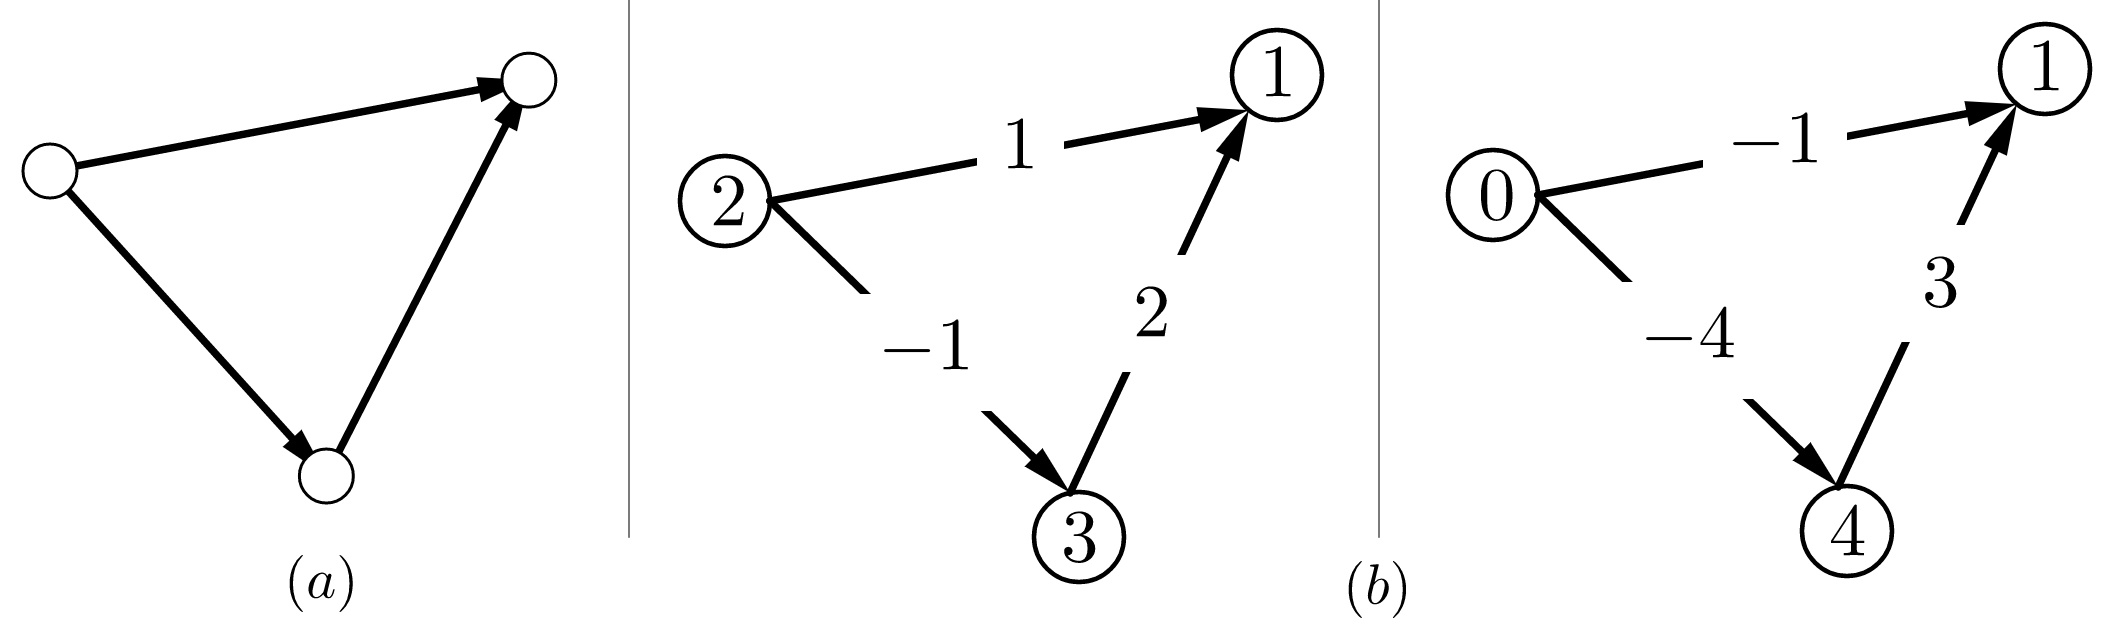
\includegraphics[scale=0.2]{img/imgchapter2/tensiones.jpg}
    \caption{}
    \label{fig:tensiones}
\end{figure}
\hfill $\blacklozenge$
\end{ejem}

\index{Espacio! de tensiones}En resumen, $\mathsf{R}(\mathbf{M})$ está conformado por todas las posibles tensiones en $D$. Luego, el conjunto de tensiones de una digráfica es un espacio vectorial llamado el \textit{espacio de tensiones de} $D$, denotado por $\mathcal{B}(D)$, es decir, $\mathcal{B}(D):=\mathsf{R}(\mathbf{M})$. 

Resulta sencillo asociar tensiones a los conjuntos de corte. En efecto, sea $\partial(X)$ un corte de $D$ y defínase $g_{\partial(X)}\colon A(D) \rightarrow \mathbb{R}$ como 
$$
g_{\partial(X)}(a) = \left\{\begin{matrix}
\quad1, & a \in \partial^{+}(X)\\ 
\ -1, & a \in \partial^{-}(X)\\
\quad 0, & a \notin \partial(X).
\end{matrix}\right.
$$
Verifiquemos que $g\in \mathsf{R}(\mathbf{M})$. Consideramos el potencial $p$ cuya de regla de correspondencia es
$$
p(v) = \left\{\begin{matrix}
1, & v \in X\\ 
0, & v \notin X.
\end{matrix}\right.
$$
Entonces 
$$
\mathbf{p}^{\textnormal{T}}\mathbf{c}_{a} = p(t(a)) - p(h(a)) = p(v) =
\left\{\begin{matrix}
\quad 1, & t(a) \in X \quad y \quad h(a) \notin X \\ 
\ -1, & h(a) \in X \quad y \quad t(a) \notin X\\
\quad 0, & \{t(a), h(a)\} \subseteq X.
\end{matrix}\right.
$$
Por consiguiente,
\begin{align*}
\mathbf{p^{\textnormal{T}}\mathbf{c}}_{a} &= \left\{\begin{matrix}
\quad1, & a \in \partial^{+}(X)\\ 
\ -1, & a \in \partial^{-}(X)\\
\quad 0, & a \notin \partial(X) 
\end{matrix}\right. 
\\ &= g_{\partial(X)}(a).
\end{align*}
De donde se concluye satisfactoriamente que $\mathbf{g}^{\textnormal{T}}_{\partial(X)} = \mathbf{p^{t}M}$ y, así, $\mathbf{g}_{\partial(X)} \in \mathcal{B}(D)$. 

\begin{ejem}
En la digráfica del inciso $(a)$ de la imagen \ref{fig:tensionesycortes} se muestra el conjunto de corte asociado a $X=\{u_{1},u_{2}\}$, mientras que en $(b)$ se encuentra la tensión que corresponde a $\partial(X)$.

\begin{figure}[H]
    \centering
    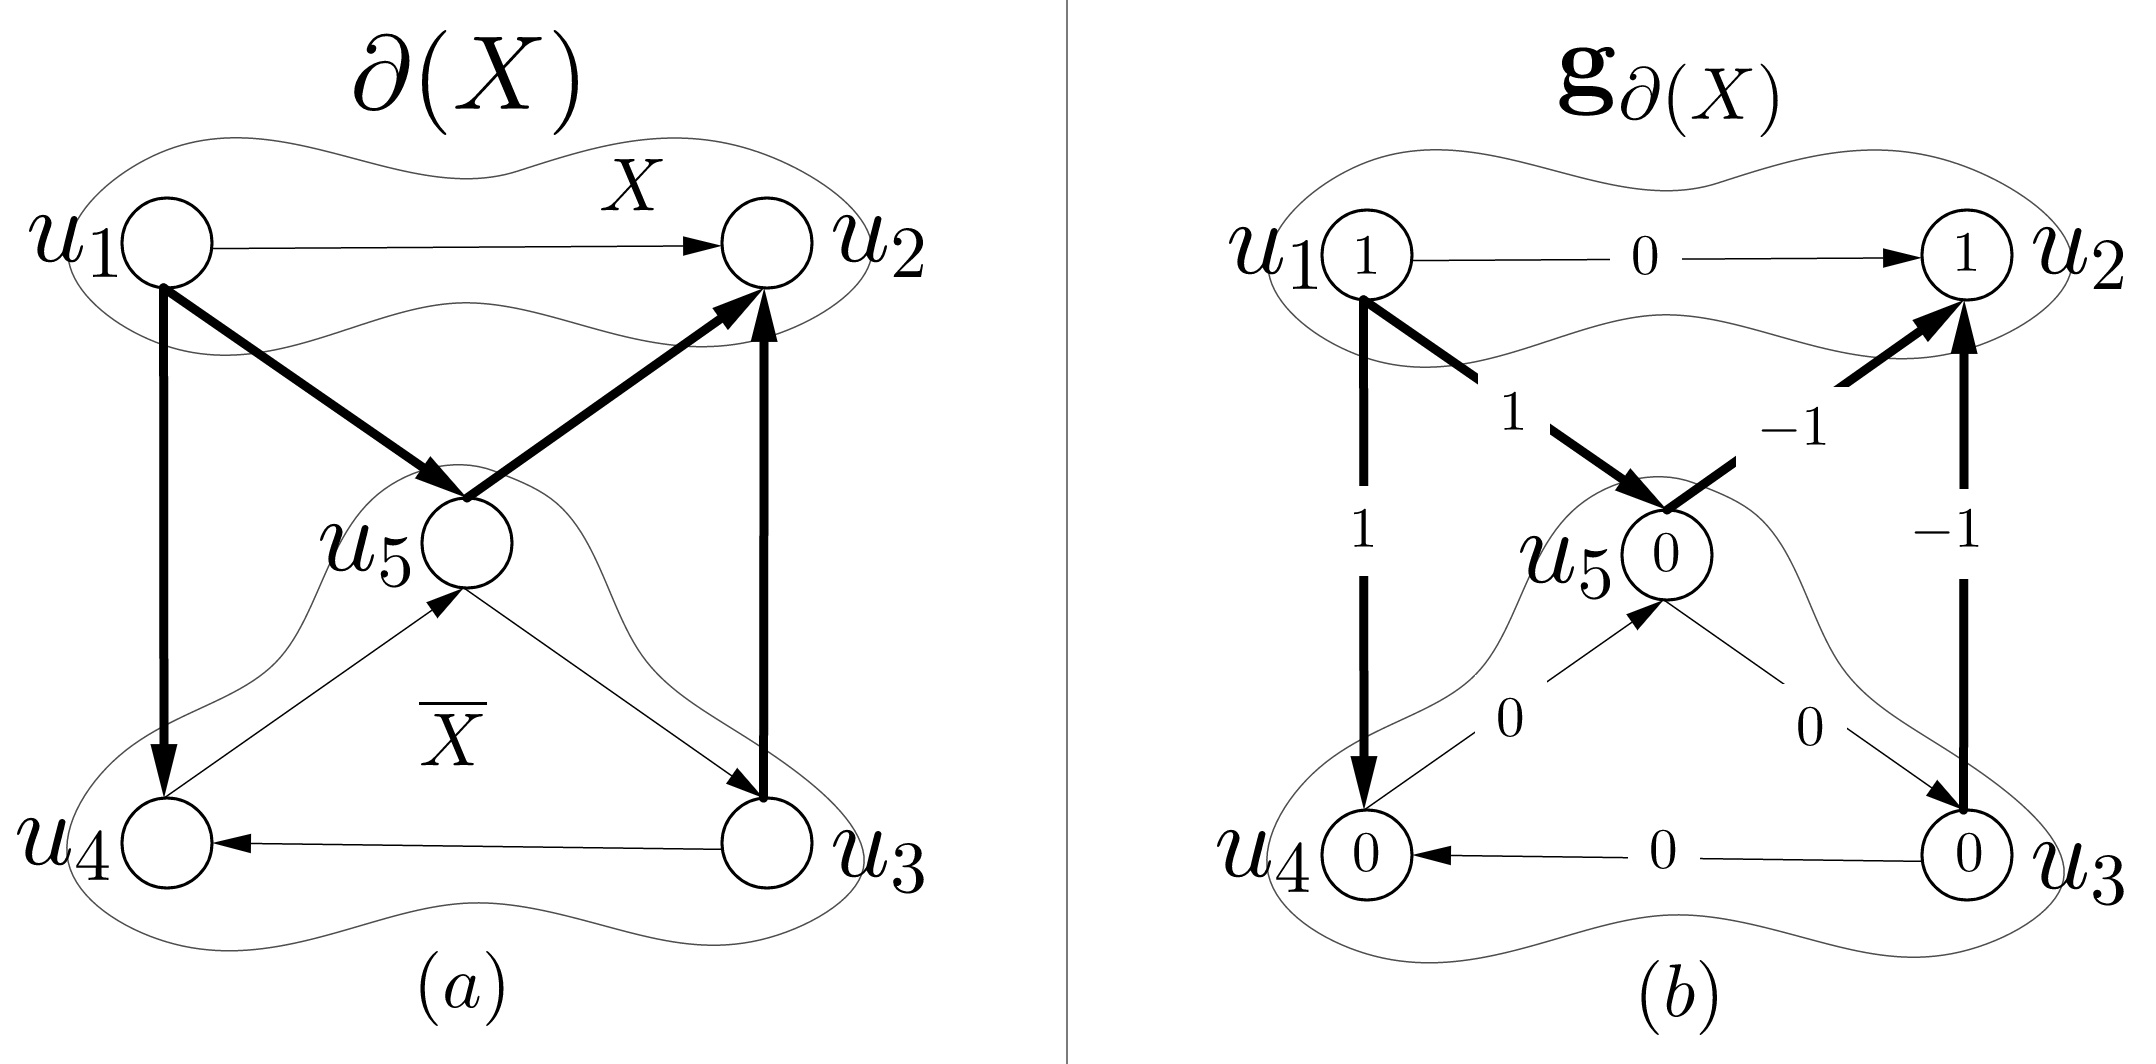
\includegraphics[scale = 0.2]{img/imgchapter2/tensionesycortes.jpg}
    \caption{}
    \label{fig:tensionesycortes}
\end{figure}
\hfill $\blacklozenge$
\end{ejem}

Con base en los párrafos anteriores, nos damos cuenta que $\mathbf{e}^{\textnormal{T}}_{i}\mathbf{M} = \mathbf{g}^{\textnormal{T}}_{\partial({u_{i})}}$, donde $\mathbf{e}^{\textnormal{T}}_{i}$ es el $i-$ésimo vector canónico de $\mathbb{R}^{n}$. Por lo que, de hecho, el vector $\mathbf{g}^{\textnormal{T}}_{\partial{(u_{i})}}$ es el $i-$ésimo  renglón de la matriz de incidencia, i.e.,
$$
\mathbf{M} = \begin{bmatrix}
\mathbf{g}^{\textnormal{T}}_{\partial(u_{1})} \\
\-- \\
\vdots \\
\--\\
\mathbf{g}^{\textnormal{T}}_{\partial(u_{n})}
\end{bmatrix}.
$$

Ahora exploraremos qué propiedades tiene las tensiones asociadas a los cortes minimales de $D$.

\begin{lema}
Supongamos que $g$ es una tensión de $D$ y que $\mathbf{g} \neq \mathbf{0}$. Entonces el soporte de $g$ contiene un conjunto de corte minimal. Más aún, si $\mathbf{g} \geq \mathbf{0}$, hay un corte minimal dirigido contenido en $supp(g)$.
\end{lema}

\begin{proof}
Dado que $\mathbf{g} \in \mathcal{B}(D)$, hay un potencial $\mathbf{p}$ tal que $\mathbf{g}^{\textnormal{T}} = \mathbf{p}^{\textnormal{T}}\textbf{M}$. Como $\mathbf{g} \neq \mathbf{0}$, entonces $supp(g) \neq \emptyset$. Así, tomemos $\alpha \in supp(g)$ haciendo $u:=t(\alpha)$ y $v:=h(\alpha)$.

Sea $X:=\{w \in V | p(w) = p(u)\}$. Afirmamos que $\partial(X) \subseteq supp(g)$. Si no sucediera, entonces existiría un arco $\beta$ en el corte asociado a $X$ que no es elemento del soporte de $g$. Esto implicaría que $g(\beta) = 0$. Si $x:=t(\beta)$ y $y:=h(\beta)$, entonces $p(x) - p(y) = 0$, es decir, $p(x) = p(y)$.

Claramente, se tendrían dos casos: $\beta \in \partial^{+}(X)$ ó $\beta \in \partial^{-}(X)$. Si se diera el primero, se tendría que $x \in X$ y $y \in \overline{X}$. Entonces $p(u) = p(x) = p(y)$ y, por definición, $ y \in X$, una contradicción. El segundo caso es análogo. Por lo tanto, es imposible que $\partial(X)\nsubseteq supp(g)$.

Debido a que $D$ es conexa, $\partial(X) \neq \emptyset$. Luego, debe existir un conjunto de corte minimal $B$ contenido en $\partial(X)$. Puesto que $\partial(X) \subseteq supp(g)$, se cumple $B \subseteq supp(g)$.

Ahora, supongamos que $\mathbf{g} \geq \mathbf{0}$. Puesto que $\mathbf{g} \geq \mathbf{0}$, se desprende inmediatamente que $$supp(g) = \{a \in A(D) | g(a)>0 \}.$$ Entonces, nótese que, para todo $a\in supp(g)$, $$g(a) = p(t(a)) - p(h(a)) > 0,$$ es decir, $p(t(a))>p(h(a))$. Esto implica que no existen ciclos dirigidos contenidos en el soporte de $g$. En efecto, asumamos que hay uno, digamos $(v_{1},\ldots,v_{l},v_{1})$. No obstante, dados los razonamientos de este párrafo, concluiríamos que $p(v_{1}) > p(v_{1})$, algo imposible. Por tanto, no hay ciclos dirigidos en $supp(g)$.

Como $supp(g)$ es una digráfica acíclica, se mencionó en el capítulo anterior que, necesariamente, debe tener al menos una fuente $w$. Por lo que $\partial(w))$ es un corte dirigido en $supp(g)$. Por una observación del capítulo anterior, $\partial^{+}(w)$ contiene un corte minimal dirigido, digamos $B^{+}$. Entonces $B^{+} \subseteq supp(g)$. 

\end{proof}

\begin{teo}  \label{teo:tensiones}
Toda tensión en $D$ es una combinación lineal de las tensiones asociadas a los cortes minimales de $D$.
\end{teo}
\begin{proof}
Supongamos que $B_{1}, \ldots, B_{q}$ son los conjuntos de corte minimales de $D$.
Sea \\$g \in \mathcal{B}(D)$. La prueba se hace por inducción fuerte sobre el número de arcos en $supp(g)$.

\underline{Paso base}. Asumimos que $|supp(g)| = 0$. Si ésto sucede, sólo resta decir que $\mathbf{g}= \mathbf{0}$ y se cumple el enunciado del teorema.

\underline{Hipótesis de inducción}. Supóngase que, para toda $q \in \mathcal{B}(D)$, si $|supp(q)|< k$, entonces $q$ es combinación lineal de las tensiones asociadas a los cortes minimales.

\underline{Paso inductivo}. Digamos ahora que $|supp(g)| = k$. Por el lema anterior, debe existir un corte minimal $\partial(X)$ contenido en el soporte de $g$. Si tomamos a $X$ de forma adecuada, debe haber un arco $\alpha^{*}$ en $\partial(X)$ tal que $g_{\partial(X)}(\alpha^{*})= 1$. 

Sea $q:=g - g(\alpha^{*})g_{\partial(X)}$. Ya que $g$ y $g_{\partial(X)}$ son elementos de $\mathcal{B}(D)$, un espacio vectorial, entonces $q \in \mathcal{B}(D)$. Además, afirmamos que $supp(q)\subsetneqq supp(g)$. Consideremos $\beta \in supp(q)$. Observemos que $g(\beta) = q(\beta) + g(\alpha^{*})g_{\partial(X)}(\beta)$. Si $\beta \notin supp(g)$, se tendría que  $g(\beta)=0$ y  $0 = q(\beta) + g(\alpha^{*})g_{\partial(X)}(\beta)$. 

Por otro lado, al no pertenecer $\beta$ al soporte de $g$, tampoco pertenecería a $\partial(X)$ y $g_{\partial(X)}(\beta) = 0$. Luego, la igualdad anterior se reduce a que $q(\beta)= 0$, una contradicción porque $\beta \in supp(q)$. Así que, efectivamente, $supp(q) \subseteq supp(g)$.

Es evidente que $\alpha^{*} \in supp(g)$ porque $\alpha^{*} \in \partial(X)$ y $\partial(X) \subseteq supp(g)$. Entonces \\$q(\alpha^{*}) = g(\alpha^{*}) - g(\alpha^{*})\cdot g_{\partial(X)}(\alpha^{*}) = g(\alpha^{*}) - g(\alpha^{*})\cdot1 = 0$. Por tanto, $\alpha^{*} \notin supp(q)$ y, con ésto, se deduce que $supp(q) \subsetneqq supp(g)$.

Los párrafos previos implican que $q \in \mathcal{B}(D)$ y $|supp(q)|<k$. De esta manera, por hipótesis de inducción, existen escalares $\lambda_{1}, \ldots, \lambda_{q} \in \mathbb{R}$ tales que 
$$
\mathbf{q} = \mathbf{g} - g(\alpha^{*})\mathbf{g}_{\partial(X)} = \sum_{i=1}^{q} \lambda_{i}\mathbf{g}_{B_{i}}.
$$
De donde
$$
\mathbf{g} = \sum_{i=1}^{q} \lambda_{i}\mathbf{g}_{B_{i}} + g(\alpha^{*})\mathbf{g}_{\partial(X)}.
$$
Recuérdese que $\partial(X)$ es un corte minimal, lo cual significa que $B_{j}=\partial(X)$, para alguna $j \in \{1, \ldots, q\}$. Entonces la igualdad anterior nos permite concluir que $\mathbf{g}$ es una combinación lineal de las tensiones asociadas a los conjuntos de corte minimales.

\end{proof}

\vspace{1cm}
\begin{cor}
El conjunto de tensiones asociadas a los cortes minimales de $D$ es un generador del espacio $\mathcal{B}(D)$.
\end{cor}

¿Qué sucede si $D$ es inconexa? Digamos que $D = \bigcup_{i=1}^{c}F_{i}$, con $F_{1}, \ldots, F_{c}$ las componentes conexas de $D$ y $c:=c(D)$ la cantidad total de sus componentes conexas. Sabemos que si ordenamos de manera adecuada los vértices y las aristas de $D$, su matriz de incidencia tiene la forma:
$$
\mathbf{M}_{D} = \begin{bmatrix}
\mathbf{M}_{F_{1}} & \cdots  & \mathbf{O} \\ 
\vdots & \ddots  & \vdots \\ 
\mathbf{O} & \cdots & \mathbf{M}_{F_{c}}
\end{bmatrix}.
$$

En otras palabras, $\mathbf{M}_{D}$ es una matriz diagonal por bloques. Aquí podemos considerar las subdigráficas generadoras $\mathcal{F}_{i}$ (cuya construcción se hizo en secciones anteriores). Entonces puede verificarse que 
$$
\mathbf{M}_{D} = \begin{bmatrix}
\mathbf{M}_{\mathcal{F}_{1}} &|& \cdots &|& \mathbf{M}_{\mathcal{F}_{1}}
\end{bmatrix}.
$$

De esta forma es claro que 

$$\mathsf{R}(\mathbf{M}_{D}) = \mathsf{R}(\mathbf{M}_{\mathcal{F}_{1}}) \oplus \cdots \oplus \mathsf{R}(\mathbf{M}_{\mathcal{F}_{c}}).$$

 Así, $$\mathsf{R}(\mathbf{M}_{D}) = \mathcal{B}(\mathcal{F}_{1}) \oplus \cdots \oplus \mathcal{B}(\mathcal{F}_{c}).$$

Por otro lado, tomemos $\mathbf{g} \in \mathsf{R}(\mathbf{M}_{D})$. Entonces existe $\mathbf{p} \in \mathbb{R}^{n}$ tal que $$\mathbf{g}^{\textnormal{T}} = \mathbf{p}^{\textnormal{T}}\mathbf{M}_{D}.$$ Dados los tamaños de las matrices, podemos partir a $\mathbf{g}$ y $\mathbf{p}$ como $\mathbf{g}^{\textnormal{T}} = \begin{bmatrix}
\mathbf{g}_{1}^{\textnormal{T}} & \cdots  & \mathbf{g}_{c}^{\textnormal{T}} 
\end{bmatrix}$ y\\ $\mathbf{p}^{\textnormal{T}} = \begin{bmatrix}
\mathbf{p}_{1}^{\textnormal{T}} & \cdots  & \mathbf{p}_{c}^{\textnormal{T}} 
\end{bmatrix}$ de tal manera que:

\begin{align*}
    \begin{bmatrix}
\mathbf{g}_{1}^{\textnormal{T}} & \cdots  & \mathbf{g}_{c}^{\textnormal{T}} 
\end{bmatrix} &= \begin{bmatrix}
\mathbf{p}_{1}^{\textnormal{T}} & \cdots  & \mathbf{p}_{c}^{\textnormal{T}} 
\end{bmatrix} \begin{bmatrix}
\mathbf{M}_{F_{1}} & \cdots  & \mathbf{O} \\ 
\vdots & \ddots  & \vdots \\ 
\mathbf{O} & \cdots & \mathbf{M}_{F_{c}}
\end{bmatrix}\\ &= \begin{bmatrix}
 \mathbf{p}_{1}^{\textnormal{T}}\mathbf{M}_{F_{1}} & \cdots &  \mathbf{p}_{c}^{\textnormal{T}}\mathbf{M}_{F_{c}}
\end{bmatrix}.
\end{align*}
De donde $\mathbf{g}_{i}^{\textnormal{T}} = \mathbf{p}_{i}^{\textnormal{T}}\mathbf{M}_{F_{i}}$, i.e., cada $\mathbf{g}_{i}$ es una tensión en $\mathcal{B}(F_{i})$. Y así, deducimos que

$$
g(a) = \left\{\begin{matrix}
g_{1}(a), & a \in A(F_{1})\\ 
\vdots & \vdots \\ 
g_{c}(a), & a \in A(F_{c})
\end{matrix}\right.
$$
y
$$
p(a) = \left\{\begin{matrix}
p_{1}(v), & v \in V(F_{1})\\ 
\vdots & \vdots \\ 
p_{c}(v), & v \in V(F_{c})
\end{matrix}\right.
$$
Es sencillo probar que $g(a) = p(t(a)) - p(h(a))$, o sea, que $g$ cumple la misma propiedad que las tensiones en digráficas conexas. Por tanto, definimos  el espacio de tensiones de $D$ como el espacio generado por los renglones de $\mathbf{M}_{D}$, $\mathcal{B}(D):=\mathsf{R}(\mathbf{M}_{D})$ (tal como en las digráficas conexas). Finalmente, por lo argumentado líneas arriba, concluimos que
$$
\mathcal{B}(D) = \mathcal{B}(\mathcal{F}_{1}) \oplus \cdots \oplus \mathcal{B}(\mathcal{F}_{c}).
$$
Los teoremas que enunciamos para digráficas conexas, involucrando al espacio de tensiones, también son válidos para aquellas que son inconexas (con sus respectivas modificaciones).


\subsection{Espacio de circulaciones $\mathcal{C}(D)$}

Ahora exploraremos el kernel de la matriz de incidencia de $D$ y describiremos la naturaleza de sus elementos. Conviene antes establecer ciertas notaciones que facilitarán nuestro estudio. 

Supongamos que $q \colon A(D) \rightarrow \mathbb{R}$. Si $S\subseteq A$, escribimos $Q(S):= \sum_{a \in S} q(a)$. En particular, si $S$ es un conjunto de corte usaremos la siguiente notación: $Q^{+}(X): = Q(\partial^{+}(X))$ y $Q^{-}(X):=Q(\partial^{-}(X))$.
  
En resumen,
$$
Q^{+}(X) =  \sum_{a \in \partial^{+}(X)} q(a) \quad y \quad
Q^{-}(X) = \sum_{a \in \partial^{-}(X)} q(a). 
$$
Analizando el producto $\mathbf{M}\mathbf{q}$ observamos que, tomando en cuenta la igualdad \ref{eq:mva} y fijando un vértice $v$, 
$$
\sum_{a \in A} m_{va}q(a) = \mathbf{g}_{\partial(v)}^{\textnormal{T}} \cdot \mathbf{q} = \sum_{a \in \partial^{+}(v)} q(a) - \sum_{a \in \partial^{-}(v)} q(a) = Q^{+}(v) - Q^{-}(v).
$$
Por lo tanto,
$$
\mathbf{M}\mathbf{q}=
    \begin{bmatrix}
Q^{+}(u_{1}) - Q^{-}(u_{1})\\ 
\vdots \\
Q^{+}(u_{n}) - Q^{-}(u_{n}) 
\end{bmatrix}.
$$
Considerando $\mathbf{f} \in Ker(\mathbf{M})$, con $f \colon A(D) \rightarrow \mathbb{R}$ y $\mathbf{f} = (f(a_{1}), \ldots, f(a_{m}))$, por la igualdad anterior vemos que 
$$
\mathbf{M}\mathbf{f}= 
\begin{bmatrix}
0 \\
\vdots\\
0
\end{bmatrix}= 
\begin{bmatrix}
F^{+}(u_{1}) - F^{-}(u_{1})\\
\vdots \\
F^{+}(u_{n}) - F^{-}(u_{n}) 
\end{bmatrix}.
$$
Por tanto, un elemento $\mathbf{f}$ del kernel de $\mathbf{M}$ tiene la propiedad de que, para todo $i \in \{1,\ldots, n\}$, $F^{+}(u_{i}) - F^{-}(u_{i}) = 0$.

Por otro lado, una \textit{circulación en} $D$ es una función $f \colon A(D) \rightarrow \mathbb{R}$ que cumple la \textit{condición de conservación} en cada vértice, es decir, 
\begin{equation} \label{eq:conservation}
    F^{+}(v) = F^{-}(v), \text{ para todo }v \in V(D).
\end{equation}
\index{Espacio! de circulaciones}La condición \ref{eq:conservation} establece que $F^{+}(v) - F^{-}(v) = 0$. Así, los elementos de $Ker(\mathbf{M})$ son circulaciones, y viceversa: las circulaciones anulan a la matriz de incidencia, esto es, que pertenecen al kernel de $\mathbf{M}$. De esta manera, el conjunto de circulaciones de $D$ es un espacio vectorial sobre $\mathbb{R}$. Lo denotamos como $\mathcal{C}(D)$ y lo llamamos el \textit{espacio de circulaciones de} $D$; o sea, $\mathcal{C}(D) : = Ker(\mathbf{M}_{D})$. 

\begin{ejem}
En la imagen \ref{fig:circulacion} están dos ejemplos de circulaciones de la digráfica del inciso $(a)$.

\begin{figure}[H]
    \centering
    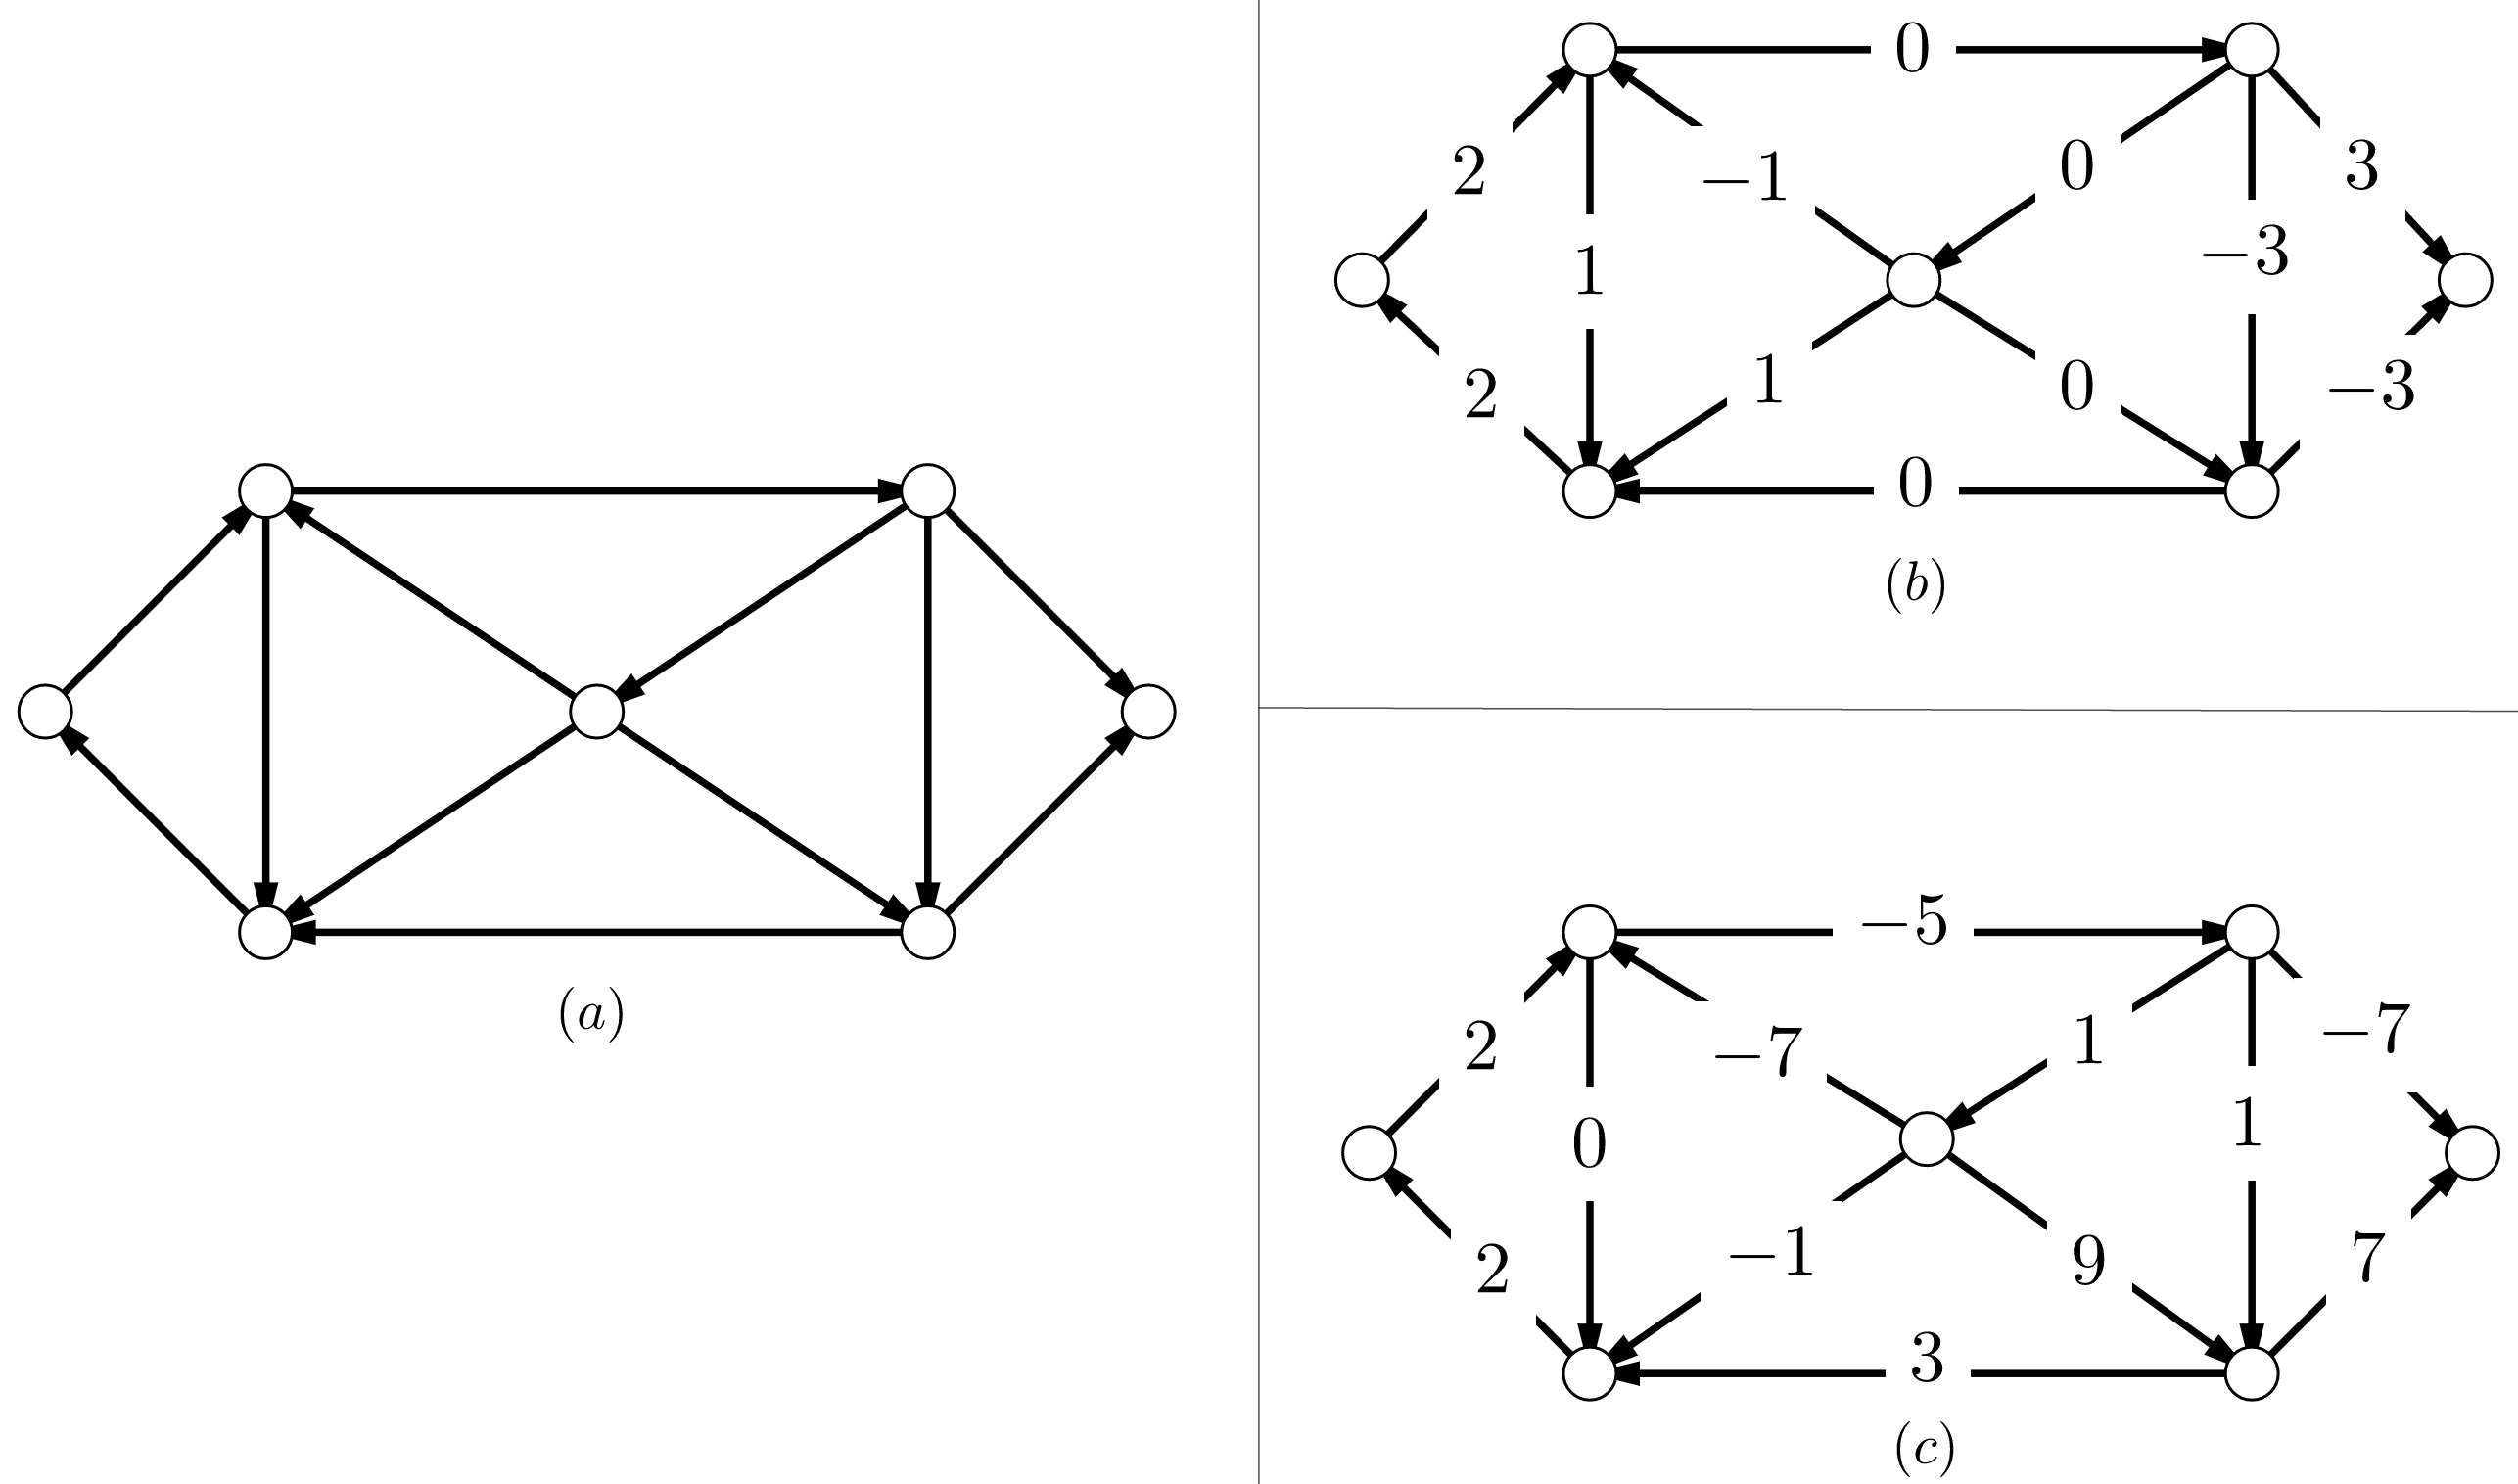
\includegraphics[scale=0.2]{img/imgchapter2/circulacion.jpg}
    \caption{}
    \label{fig:circulacion}
\end{figure}
\hfill $\blacklozenge$
\end{ejem}


Hay una manera de asociar circulaciones a los ciclos de la digráfica. Supongamos que $C$ es un ciclo contenido en $D$. Recordemos que en el capítulo $1$ mencionamos que $C$ puede ser recorrido, esencialmente, en dos direcciones: en sentido horario o en sentido antihorario (dependiendo del diagrama que representa al ciclo y de cómo se etiquetan los vértices). También comentamos que, al elegir un sentido para recorrer el ciclo, aquél induce dos subdigráficas de $C$:  la de los arcos hacia adelante $C^{+}$ y la de los arcos hacia atrás $C^{-}$.

Dicho lo anterior, escogemos un sentido para $C$ y hacemos $f_{C} \colon A(D) \rightarrow \mathbb{R}$ dada por:
$$
f_{C}(a)=\left\{\begin{matrix}
\quad 1, & a \in A(C^{+}) \\ 
\ -1, & a \in A(C^{-})\\ 
\quad 0, &a \notin A(C).
\end{matrix}\right.
$$
Veamos por qué, de hecho, $f_{C}$ es una circulación. Consideremos un vértice $v$ de $D$. Ya que $f_{C}$ se anula en arcos que no pertenecen a $C$, obtenemos que
\begin{equation} \label{eq:cortescicloscasos}
    \begin{split}
               F^{+}(v) - F^{-}(v) &= \sum_{a \in \partial^{+}(v)} f_{C}(a) - \sum_{a \in \partial^{-}(v)} f_{C}(a) \\
    &= \sum_{a \in \partial^{+}(v) \cap A(C)} f_{C}(a) - \sum_{a \in \partial^{-}(v) \cap A(C)} f_{C}(a) \\
    &= \sum_{a \in \partial(v) \cap A(C)} f_{C}(a).
    \end{split}
\end{equation}
Como sabemos que $|\partial(v) \cap A(C)| = 2$, asumiremos que $\partial(v) \cap A(C) = \{\alpha, \beta\}$. Entonces, escogiendo de antemano un sentido de recorrido para el ciclo $C$, tenemos cuatro casos (véase la figura \ref{fig:casoscortesciclos}). 
 \begin{figure}[H]
%\vspace{-1.1cm}
\centering
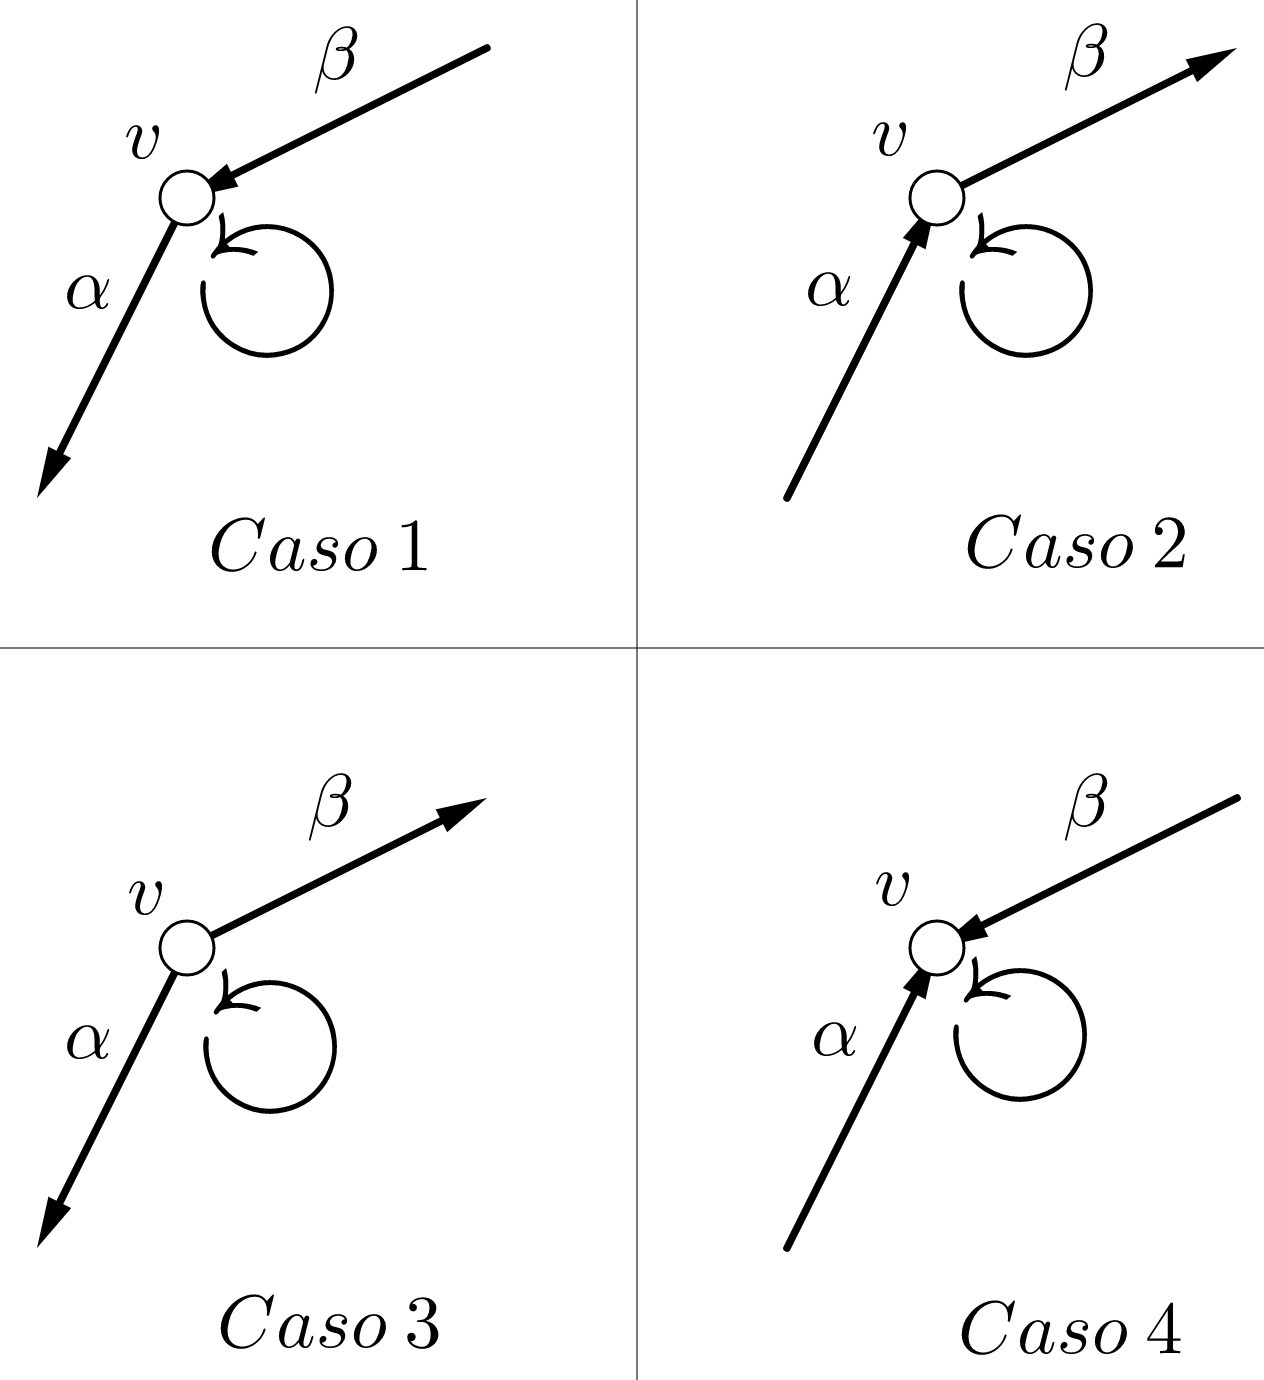
\includegraphics[scale=0.2]{img/imgchapter2/digraficacicloscasos.jpg}
\caption{}
\label{fig:casoscortesciclos}
\end{figure}
\begin{itemize}
   \item \underline{Caso 1.}  \textit{Que $\alpha \in \partial^{+}(X)$ y $\beta \in \partial^{-}(X)$}. Aquí $f_{C} (\alpha)= f_{C}(\beta) = 1.$

\item {Caso 2.} \textit{Que $\alpha \in \partial^{-}(X)$ y $\beta \in \partial^{+}(X)$}. Tenemos que $f_{C} (\alpha)= f_{C}(\beta) = -1$.

\item {Caso 3.} $\{\alpha, \beta\} = \partial^{+}(v) \cap A(C)$. Deducimos que $f_{C}(\alpha)=1$ y $f_{C}(\beta)=-1.$

\item {Caso 4.} $\{\alpha, \beta\} = \partial^{-}(v) \cap A(C)$. Puede verificarse que $f_{C}(\alpha)= -1$ y $f_{C}(\beta)=1.$ 
\end{itemize}


De todos los casos, puede verificarse que la identidad \ref{eq:cortescicloscasos} es siempre igual a $0$. Con el otro sentido de $C$ se pueden deducir otros cuatro casos que nos arrojarán los mismos resultados. Dicho de otro modo, la igualdad \ref{fig:casoscortesciclos} implica que $F^{+}(v) - F^{-}(v) = 0$, para cualquier vértice $v$. Luego entonces, $f_{C} \in \mathcal{C}(D)$. 

\begin{ejem}
En el inciso $(a)$ de la figura \ref{fig:circulacionciclo} mostramos un ciclo de la gráfica de la imagen \ref{fig:circulacion}, con la respectiva orientación (en sentido contrario a las manecillas del reloj) que hemos escogido; y en $(b)$ se halla la circulación asociada a dicho ciclo.
\begin{figure}[H]
    \centering
    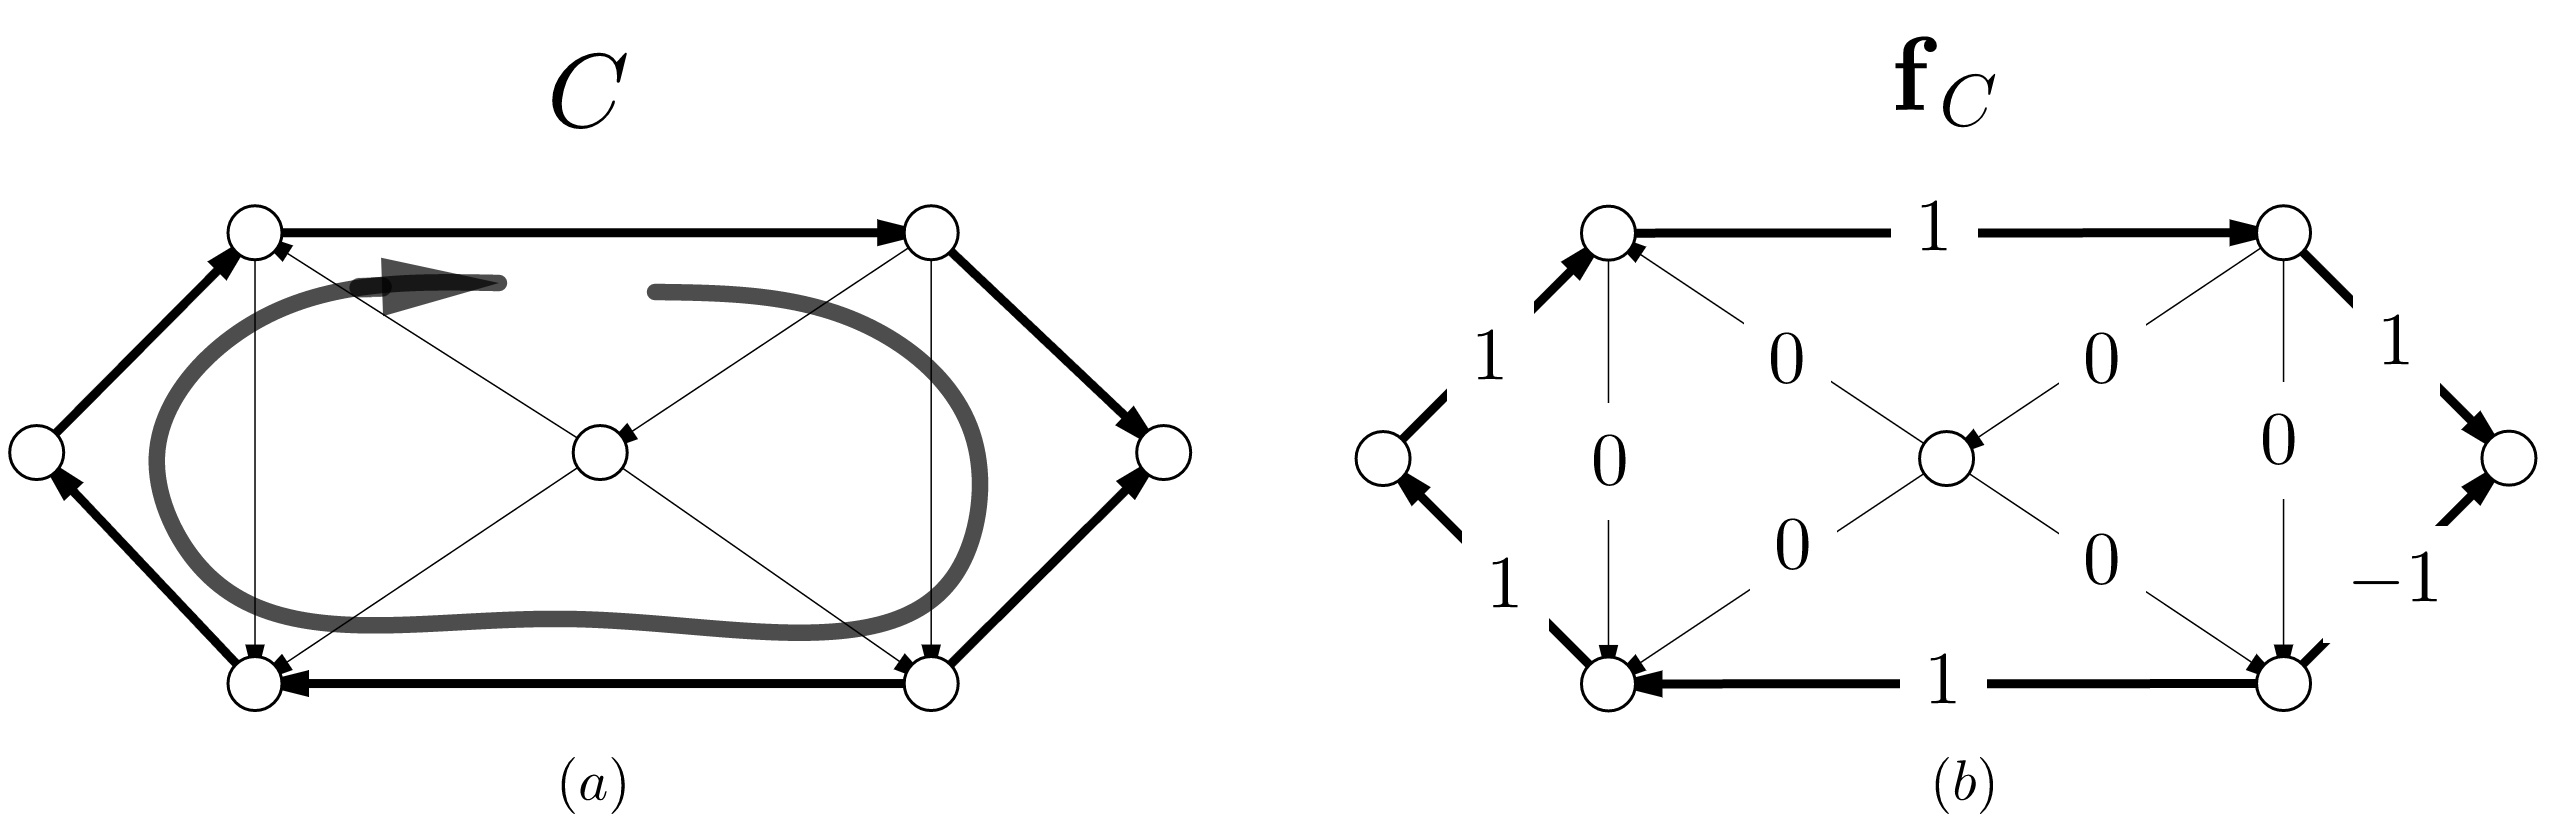
\includegraphics[scale=0.19]{img/imgchapter2/circulacionciclo.jpg}
    \caption{}
    \label{fig:circulacionciclo}
\end{figure}
\hfill $\blacklozenge$
\end{ejem}

Similarmente a como lo hicimos con las tensiones, veamos qué propiedades tienen las circulaciones asociadas a ciclos.

\begin{lema} \label{lema:circulacion}
Sea $\mathbf{f} \in \mathcal{C}(D)$. Si $\mathbf{f} \neq \mathbf{0}$, entonces hay un ciclo de $D$ contenido en $supp(f)$. Más aún, si $\mathbf{f} \geq \mathbf{0}$, entonces el soporte de $f$ contiene un ciclo dirigido.
\end{lema}

\begin{proof}
Supongamos que $\mathbf{f} \neq \mathbf{0}$. Para llegar a una contradicción, asumamos que $supp(f)$ no contiene ciclos. Entonces, apoyados de la proposición \ref{prop:hojas}, sabemos que hay un vértice $v$ de grado $1$ en $supp(f)$. Digamos que $\alpha \in supp(f)$ es el único arco incidente en $v$. Así, hay dos casos: $d_{supp(f)}^{+}(v) = 1$ ó $d_{supp(f)}^{-}(v)=1$.

Si $d_{supp(f)}^{+}(v) = 1$, entonces $\partial_{supp(f)}^{+}(v) = \{\alpha\}$ y $\partial_{supp(f)}^{-}(v) = \emptyset$. Luego, al ser $f$ una circulación, se tiene
$$
F^{+}(v) = f(\alpha) = 0 = F^{-}(v).
$$
Pero esto es una contradicción pues $\alpha \in supp(f)$ y, por definición, $f(\alpha) \neq 0$. El caso cuando $d_{supp(f)}^{-}(v)=1$ es totalmente análogo. Por tanto, $supp(f)$ contiene un ciclo.

Supongamos que $\mathbf{f} \geq \mathbf{0}$ y, ahora, que $supp(f)$ es acíclica. Debido a lo comentado en el segundo capítulo respecto a digráficas acíclicas, sabemos que $supp(f)$ tiene una fuente $u$, es decir, que $\partial_{supp(f)}^{-}(u)=\emptyset$ y $\partial_{supp(f)}^{+}(u) \neq \emptyset$. Puesto que $\mathbf{f} \geq \mathbf{0}$, se desprende inmediatamente que $supp(f) = \{a \in A(D) | f(a)>0 \}$. Entonces nótese que, como $ \partial_{supp(f)}^{+}(u) \subseteq supp(f)$, entonces $f(a) > 0$, para toda $a \in \partial_{supp(f)}^{+}(u)$. Por otro lado, 
$$
F^{+}(u)= \sum_{a \in \partial_{supp(f)}^{+}(u)} f(a)= F^{-}(u) = 0.
$$

La igualdad anterior implica, necesariamente, que $f(a) = 0$, para cualquier arco $a$ en $\partial_{supp(f)}^{+}(u)$. Esto es una contradicción. Luego, $supp(f)$ no tiene ni pozos ni fuentes y, por lo tanto, debe contener un ciclo dirigido.

\end{proof}

\begin{teo}
Toda circulación es una combinación lineal de las circulaciones asociadas a los ciclos de $D$.
\end{teo}

\begin{proof}
La prueba se realiza por inducción fuerte sobre el número de elementos del soporte de $f$ y es análoga a la demostración del teorema \ref{teo:tensiones}.
\end{proof}

\begin{cor}
El conjunto de circulaciones asociadas a los ciclos de $D$ es un generador del espacio $\mathcal{C}(D)$.
\end{cor}

Veamos qué sucede si $D$ es inconexa. Al igual que la sección pasada, suponemos que $G =  \bigcup_{i=1}^{c}F_{i}$,y tomamos las subgráficas $\mathcal{F_{i}}$. Sabemos ya del capítulo $1$ que 
$$
Ker(\mathbf{M}_{D}) = Ker(\mathbf{M}_{\mathcal{F}_{1}}) \oplus \cdots \oplus Ker(\mathbf{M}_{\mathcal{F}_{c}}).
$$

Como,  $Ker(\mathbf{M}_{\mathcal{F}_{i}}) = \mathcal{C}(\mathcal{F}_{i})$, entonces $$Ker(\mathbf{M}_{D}) = \mathcal{C}(\mathcal{F}_{1}) \oplus \cdots \oplus \mathcal{C}(\mathcal{F}_{c}).$$ Si, por otro lado, tomamos $\mathbf{f} \in Ker(\mathbf{M}_{D})$ y lo partimos según los tamaños de las submatrices, tenemos:
\begin{align*}
    \mathbf{M}_{D}\mathbf{f} = \begin{bmatrix}
\mathbf{M}_{F_{1}} & \cdots  & \mathbf{O} \\ 
\vdots & \ddots  & \vdots \\ 
\mathbf{O} & \cdots & \mathbf{M}_{F_{c}}
\end{bmatrix} \begin{bmatrix}
\mathbf{f}_{1}\\
\vdots\\ 
\mathbf{f}_{c}
\end{bmatrix} = \begin{bmatrix}
\mathbf{0}\\
\vdots\\ 
\mathbf{0}
\end{bmatrix}.
\end{align*}

Entonces $\mathbf{M}_{F_{i}}\mathbf{f}_{1} = \mathbf{0}$, es decir, $\mathbf{f}_{i}$ es una circulación en $\mathcal{C}(F_{i})$, de donde 
$$
F^{+} = \left\{\begin{matrix}
F^{+}_{1}(v), & v \in V(F_{1}) \\
\vdots & \vdots \\
F^{+}_{c}(v), & v \in V(F_{c})    
\end{matrix}\right.,
$$
y
$$
F^{-} = \left\{\begin{matrix}
F^{-}_{1}(v), & v \in V(F_{1}) \\
\vdots & \vdots \\
F^{-}_{c}(v), & v \in V(F_{c})    
\end{matrix}\right..
$$
Por lo tanto, como cada $\mathbf{f}_{i}$ es una circulación, $F^{+}(v) - F^{-}(v) = 0$. Esto sugiere que los elementos en $Ker(\mathbf{M}_{D})$ se comportan como las circulaciones en digráficas conexas. De esta manera, definimos $\mathcal{C}(D) := Ker(\mathbf{M}_{D})$ el espacio de circulaciones de $D$ como el kernel de su matriz de incidencia. Luego, $$\mathcal{C}(D) = \mathcal{C}(\mathcal{F}_{1}) \oplus \cdots \oplus \mathcal{C}(\mathcal{F}_{c}).$$ Además, los teoremas que dimos para digráficas conexas, involucrando el espacio de circulaciones, permanecen verdaderos para digráficas inconexas (con sus respectivas modificaciones).

\subsection{Relación entre $\mathcal{B}(D)$ y $\mathcal{C}(D)$}

Sabemos del primer capítulo que $(\mathsf{R}(\mathbf{M}))^{\perp}=Ker(\mathbf{M})$ y que $(Ker(\mathbf{M}))^{\perp} = \mathsf{R}(\mathbf{M})$.

Por lo tanto, $(\mathcal{B}(D))^{\perp} = \mathcal{C}(D)$ y $(\mathcal{C}(D))^{\perp} = \mathcal{B}(D)$, es decir, los espacios de tensiones y circulaciones son complementos ortogonales.

Luego, necesariamente $\mathcal{B}(D) \cap \mathcal{C}(D) = \{\mathbf{0}\}$. Ninguna tensión puede ser al mismo tiempo una circulación y viceversa. Nótese que lo que acabamos de mencionar no ocurría con los espacios de cortes y de ciclos de las gráficas no dirigidas. En conclusión, $\mathbb{R}^{m} = \mathcal{B}(D) \oplus \mathcal{C}(D)$.

\subsection{Rango, nulidad y relaciones de independencia lineal en $\mathbf{M}_{D}$}

En digráficas hay un resultado similar al teorema \ref{teo:liaciclicas} y muchas de las ideas que presentamos en esa sección se siguen cumpliendo. Si $H$ es una subdigráfica generadora de $D$,  sucede que $\mathbf{M}_{H}$ es una submatriz de $\mathbf{M}_{D}$, pues conservan los mismos renglones (vértices) y las columnas de $\mathbf{M}_{H}$ corresponden a $A(H)\subseteq A(D)$.

Si $A(D)=\{a_{1}, \ldots, a_{m}\}$, $\mathbf{c}_{e}$ es la columna de $\mathbf{M}$ que corresponde al arco $e$. Entonces:
$$
\mathbf{M}=\begin{bmatrix}
\mathbf{c}_{a_{1}} |& \cdots & |\mathbf{c}_{a_{m}} 
\end{bmatrix}.
$$
Notemos ahora que si $S \subseteq A(D)$, entonces $\mathbf{M}_{D[S]}$ es la submatriz $\begin{bmatrix}
\mathbf{c}_{a}  
\end{bmatrix}_{a \in S}$ de $\mathbf{M}_{D}$.

\begin{teo}\label{teo:liaciclicas2} Si $S \subseteq A(D)$, entonces
el conjunto de columnas $\{\mathbf{c}_{a} | a \in S\}$ es linealmente independiente si y sólo si $D[S]$ es acíclica.
\end{teo}

\begin{proof}
Para probar la\textit{necesidad}, supongamos que $\{\mathbf{c}_{a} | a \in S\}$ es linealmente independiente y, para llegar a una contradicción, que hay un ciclo $\Gamma$ en $D[S]$ y consideremos su circulación asociada $f_{\Gamma}$. 

Entonces $$\mathbf{M}_{D[S]}\cdot\mathbf{f}_{\Gamma}= \mathbf{0}.$$ No obstante, esto implica que $\sum_{a \in S} f_{\Gamma}(a)\cdot\mathbf{c}_{a} = \mathbf{0}$. Como $\{\mathbf{c}_{a} | a \in S\}$ es linealmente independiente, se tiene que $f_{\Gamma}(a) = 0$, para toda $a \in S$. Luego, $\mathbf{f}_{\Gamma} = \mathbf{0}$ es la circulación trivial y esto implica que el ciclo $\Gamma$ en realidad es vacío (una contradicción). En consecuencia, $D[S]$ es acíclica.

Ahora, para la \textit{suficiencia}, asumamos que $D[S]$ es acíclica. Tomemos una combinación lineal cualquiera de $\{\mathbf{c}_{a} | a \in S\}$, digamos $\sum_{a \in S} \lambda_{a} \mathbf{c}_{a} = \mathbf{0}$, con $\lambda_{a} \in \mathbb{R}$.

La igualdad anterior implica que $\mathbf{M}_{D[S]}\boldsymbol{\lambda} = \mathbf{0}$, donde $\boldsymbol{\lambda}$ es el vector cuyas entradas son $\lambda_{a}$.

Entonces, $\boldsymbol{\lambda} \in Ker(\mathbf{M}_{D[S]}) = \mathcal{C}(D[S]) = \{\mathbf{0}\}$, porque $G[S]$ es acíclica y su única circulación posible es la trivial. Así, $\boldsymbol{\lambda} = \mathbf{0}$ y, en consecuencia, $\lambda_{a} = 0$, para toda $a \in S$. Por lo tanto, $\{\mathbf{c}_{a} | a \in S\}$ es linealmente independiente.

\end{proof}
 
 Varias implicaciones se siguen de este importante teorema. Es claro que si $T$ es un bosque generador maximal de $D$, entonces $T$ es una subdigráfica acíclica contenida en $D$ más grande posible. De esta forma $\{\mathbf{c}_{a} | a \in A(T)\}$ es el conjunto linealmente independiente más grande posible en $\mathsf{C}(\mathbf{M})$ y, por consiguiente, es una base para este espacio de columnas. Puesto que $\{\mathbf{c}_{a} | a \in A(T)\}$ tiene $n-c$ columnas (pues $T$ tiene $n-c$ arcos), entonces $\dim(\mathsf{C}(\mathbf{M})) = n- c$. Sin embargo, esta también es la dimensión del espacio generado por los renglones $\mathsf{R}(\mathbf{M})$. Como $\mathcal{B}(D) = \mathsf{R}(\mathbf{M})$, concluimos que el espacio de tensiones de $D$ tiene dimensión $n - c$; y debido al teorema de la dimensión, \\$\dim(Ker(\mathbf{M}))= m - n + c$, es decir, $m - n + c$ es la dimensión del espacio de circulaciones de $D$. Esto, a su vez, tiene otra conclusión principal respecto a la matriz de incidencia que dejamos establecida en el siguiente teorema. 
 
 \begin{teo}
 Se tiene que $\dim(\mathcal{B}(D)) = n - c$ y $\dim(\mathcal{C}(D)) = m - n + c$. Por lo tanto, $rank(\mathbf{M_{D}}) = n - c$ y $null(\mathbf{M}_{D}) = m - n + c$.
 \end{teo}
 
 Definimos el rango y la nulidad de $D$, respectivamente, como los números $\rho(D):=rank(\mathbf{M}_{D}) = n -c$  y $\mu(D):=\null(\mathbf{M}_{D}) = m - n + c$.
 
 El lector atento también podrá imaginarse que, al igual que con las gráficas, las bases del espacio de columnas están estrechamente ligadas con los bosques generadores maximales.
 
\begin{cor} Sea $S\subseteq A(D)$. Entonces $\{\mathbf{c}_{a} | a \in S \}$ es una base para el espacio de columnas $\mathsf{C}(\mathbf{M}_{D})$ si y sólo si $D[S]$ es un bosque generador maximal. Por lo tanto, las bases de $\mathsf{C}(\mathbf{M}_{D})$ están en correspondencia uno a uno con los bosques generadores maximales de $D$.
\end{cor} 

Por último, dado $S \subseteq A(D)$, los resultados previos implican que \textit{$D[S]$ contiene un ciclo si y sólo si $\{\mathbf{c}_{a} | a \in S\}$ es un conjunto linealmente dependiente.} 

\subsection{Matrices reducidas}

He aquí otra observación: ya se había mencionado que en cada columna sólo hay dos entradas: un ``$1$'' y un ``$-1$''. Esto implica que la suma de todos los renglones de $\mathbf{M}$ sea igual al vector $\mathbf{0}$. En otros términos, tenemos que:
$$
\sum_{i = 1}^{n} \mathbf{g}_{\partial(u_{i})} = \mathbf{0}.
$$

Lo que nos permite despejar cualquier renglón y ponerlo en combinación lineal del resto:
$$
\mathbf{g}_{\partial(u_{j})} = \sum_{i \neq j} -\mathbf{g}_{\partial(u_{i})}.
$$

Esta última igualdad nos permite definir \textit{matrices de incidencia reducidas} para digráficas, de una manera parecida a como lo hicimos para las gráfica no orientadas: si $D$ es conexa, entonces $\widehat{\mathbf{M}}_{D}$ es la matriz que resulta de remover cualquier renglón de $D$; si $D$ no es conexa, entonces $\widehat{\mathbf{M}}_{D}$ es la matriz que resulta de eliminar un renglón cualquiera de cada submatriz correspondiente a su respectiva componente conexa. Por ejemplo, las matrices de incidencia reducidas de los bosques serán matrices cuadradas de tamaño $(n - c) \times (n - c)$. Los razonamientos anteriores nos permiten afirmar lo siguiente.

\begin{prop} \label{prop:rango2}
En $\mathbb{R}$, se cumple que $rank(\widehat{\mathbf{M}}_{D}) = rank(\mathbf{M}_{D})= n-c$. En particular, la matriz de incidencia reducida de todo bosque $T$ es una matriz no singular, es decir, $\det(\widehat{\mathbf{M}}_{T}) \neq 0$.
\end{prop}

Aún más, de la proposición anterior y el teorema \ref{teo:liaciclicas2} se deduce un corolario más.

\begin{cor}
Toda submatriz cuadrada, de tamaño $(n-c) \times (n-c)$, de la matriz de incidencia de $G$ es no singular si y sólo si es la matriz de incidencia reducida de algún bosque generador maximal de $T$.
\end{cor}
 

\section{Cortes y ciclos fundamentales en digráficas}
Hasta el momento conocemos la dimensión de los espacios $\mathcal{B}(D)$ y $\mathcal{C}(D)$ e incluso aprendimos que las tensiones asociadas a cortes minimales y las circulaciones correspondientes a ciclos conformaban conjuntos generadores para dichos espacios. No obstante, todavía no hallamos sus bases. 

En gráficas no dirigidas, los cortes y ciclos fundamentales resultan ser de gran utilidad pues son bases para los espacios de corte y de ciclos, respectivamente. Veremos en esta sección cómo estos cortes y ciclos especiales nos permitirán construir sencillamente unas bases para los espacios $\mathcal{B}(D)$ y $\mathcal{C}(D)$.

\subsection{Tensiones fundamentales}
Supongamos primero que $D$ es conexa. Sea $T$ un árbol generador de $D$. Entonces $T$ define (en la forma como lo hicimos en el capítulo $2$) $n-1$ conjuntos de cortes fundamentales en $G[D]$, la gráfica subyacente de $D$. Considerando las direcciones de las aristas, también diremos que estos conjuntos son \textit{cortes fundamentales de $D$ asociados a $T$}.

En secciones previas, vimos a cualquier conjunto de corte se le puede asociar una tensión de $D$. En particular, también sucede con los cortes fundamentales.

\index{Tensión! fundamental}Sea $b \in A(T)$ y consideremos $\mathscr{B}_{b}$ su corte fundamental correspondiente. Entonces la tensión asociada $\mathbf{g}_{\mathscr{B}_{b}}$ la escogemos de tal forma que $g_{\mathscr{B}_{b}}(b) = 1$ y le llamamos la \textit{tensión fundamental de $D$ con respecto a $b$ y a $T$}. Véase la figura \ref{fig:tensionescirculacionesfund}.

Ahora bien, supóngase que se ordenan los arcos de $D$ de tal manera que $$A(D) = \{b_{1}, \ldots, b_{\rho}, c_{1}, \ldots, c_{\mu}\},$$ con $A(T) = \{b_{1}, \ldots, b_{\rho}\}$ y $A(\overline{T}) = \{c_{1}, \ldots, c_{\mu}\}$. Por otro lado, consideremos todos las tensiones fundamentales de $T$ y formamos una matriz $\mathbf{B}_{f}$ en la que cada renglón es una tensión fundamental, es decir, 
$$
\mathbf{B}_{f} := \begin{bmatrix}
\mathbf{g}_{\mathscr{B}_{b_{1}}}^{\textnormal{T}} \\
\-- \\
\vdots \\
\-- \\
\mathbf{g}_{\mathscr{B}_{b_{\rho}}}^{\textnormal{T}}
\end{bmatrix}.
$$

Recordemos que  $\mathscr{B}_{b} \cap A(T) = \{b\}$ y $b$ es el único arco con esta propiedad. Esto implica que, en la matriz $\mathbf{B}_{f}$, las columnas que corresponden a las ramas de $T$ sólo tienen un ``$1$'' en el renglón de la tensión fundamental asociada a $b$.  

Por tanto, considerando el orden que le dimos a los arcos de $D$, la matriz $\mathbf{B}_{f}$ es de la forma:
$$
\mathbf{B}_{f} = \begin{bmatrix}
\mathbf{I}_{\rho} & \mathbf{K} 
\end{bmatrix}.
$$
Luego, $rank(\mathbf{B}_{f}) = \rho = n-1$. Ya que hay $n -1$ renglones en $\mathbf{B}_{f}$, entonces éstos son linealmente independientes. Esto es, que el conjunto de tensiones fundamentales  $\{\mathbf{g}_{\mathscr{B}_{b_{1}}}, \ldots, \mathbf{g}_{\mathscr{B}_{b_{\rho}}} \}$ es linealmente independiente. Dado que $\dim(\mathcal{B}(D)) = n -1$, concluimos que el conjunto de tensiones fundamentales es una base de $\mathcal{B}(D)$.

En el caso que $D = \bigcup_{i = 1}^{c} F_{i}$ sea inconexa, consideramos  un bosque generador maximal $T$ y las digráficas $\mathcal{F}_{i}$. Se toma la base de tensiones fundamentales con respecto a $T$, digamos $\gamma_{i}$, de cada $\mathcal{F}_{i}$. Como $\mathcal{B}(D) = \mathcal{B}(\mathcal{F}_{1}) \oplus \cdots \oplus \mathcal{B}(\mathcal{F}_{c})$, entonces sabemos que $\gamma = \bigcup_{i =1}^{c}\gamma_{i}$ es una base para $\mathcal{B}(D)$, con $n - c$ elementos.


\subsection{Circulaciones fundamentales}
El procedimiento que seguimos aquí es muy parecido al de la subsección anterior. Los ciclo fundamentales de $D$ son aquellos correspondientes a su gráfica subyacente. 

\index{Circulación! fundamental}Sea $c \in A(\overline{T})$ y consideramos su ciclo fundamental con respecto a $T$.  Tomamos su circulación asociada $\mathbf{f}_{\mathscr{C}_{c}}$ con la orientación tal que $f_{\mathscr{C}_{c}}(c)=1$ y la llamamos \textit{circulación fundamental de $D$ con respecto a $T$}. Véase la figura \ref{fig:tensionescirculacionesfund}.

Ordenamos los arcos de $D$ de al forma que $A(D) = A(\overline{T}) \cup A(T) $ con $A(\overline{T}) = \{c_{1}, \ldots, c_{\mu}\}$ y $A(T) = \{b_{1}, \ldots, b_{\rho}\}$. Acomodamos las circulaciones fundamentales como renglones de una matriz $\mathbf{C}_{f}$ de tal manera que:

$$
\mathbf{C}_{f} := \begin{bmatrix}
\mathbf{f}_{\mathscr{C}_{c_{1}}}^{\textbf{T}} \\
\-- \\
\vdots \\
\-- \\
\mathbf{f}_{\mathscr{C}_{c_{\mu}}}^{\textbf{T}}
\end{bmatrix}.
$$

De nuevo, nos damos cuenta que $\mathscr{C}_{c} \cap \overline{T} = c$ y es el único ciclo fundamental con esa propiedad. Esto implica que en la columna de $\mathbf{B}_{f}$ que corresponde a $c$ habrá un sólo ``$1$'', en el renglón de la respectiva circulación fundamental.

Luego, gracias al orden que le dimos a los arcos de $D$, la matriz $\mathbf{B}_{f}$ tiene la forma:
$$
\mathbf{C}_{f} = \begin{bmatrix}
\mathbf{I}_{\mu} & \mathbf{L} 
\end{bmatrix}.
$$
Por consiguiente, $rank(\mathbf{C}_{f}) = \mu = m - n + 1$. Esto implica que las $m - n +1$ circulaciones fundamentales son linealmente independientes. Como $\dim(\mathcal{C}(D)) = m - n +1$, se sigue que $\{\mathscr{C}_{c_{1}}, \ldots, \mathscr{C}_{c_{\mu}}\}$ es una base para el espacio de circulaciones de $D$.

En el caso que $D = \bigcup_{i = 1}^{c} F_{i}$ sea inconexa (y de manera muy similar a las tensiones) consideramos  un bosque generador maximal $T$ y se toma la base de circulaciones fundamentales con respecto a $T$, digamos $\gamma_{i}$, de cada subdigráfica $\mathcal{F}_{i}$. Como $\mathcal{C}(D) = \mathcal{C}(\mathcal{F}_{1}) \oplus \cdots \oplus \mathcal{C}(\mathcal{F}_{c})$, entonces sabemos que $\gamma = \bigcup_{i =1}^{c}\gamma_{i}$ es una base para $\mathcal{C}(D)$, con $m - n + c$ elementos.

\begin{ejem}
En la figura \ref{fig:tensionesycortes} representamos un árbol generador de $K_{4}$. En $(b)$ colocamos una tensión y una circulación fundamentales respecto a los arcos $f$ y $b$, respectivamente. 

\begin{figure}[H]
    \centering
    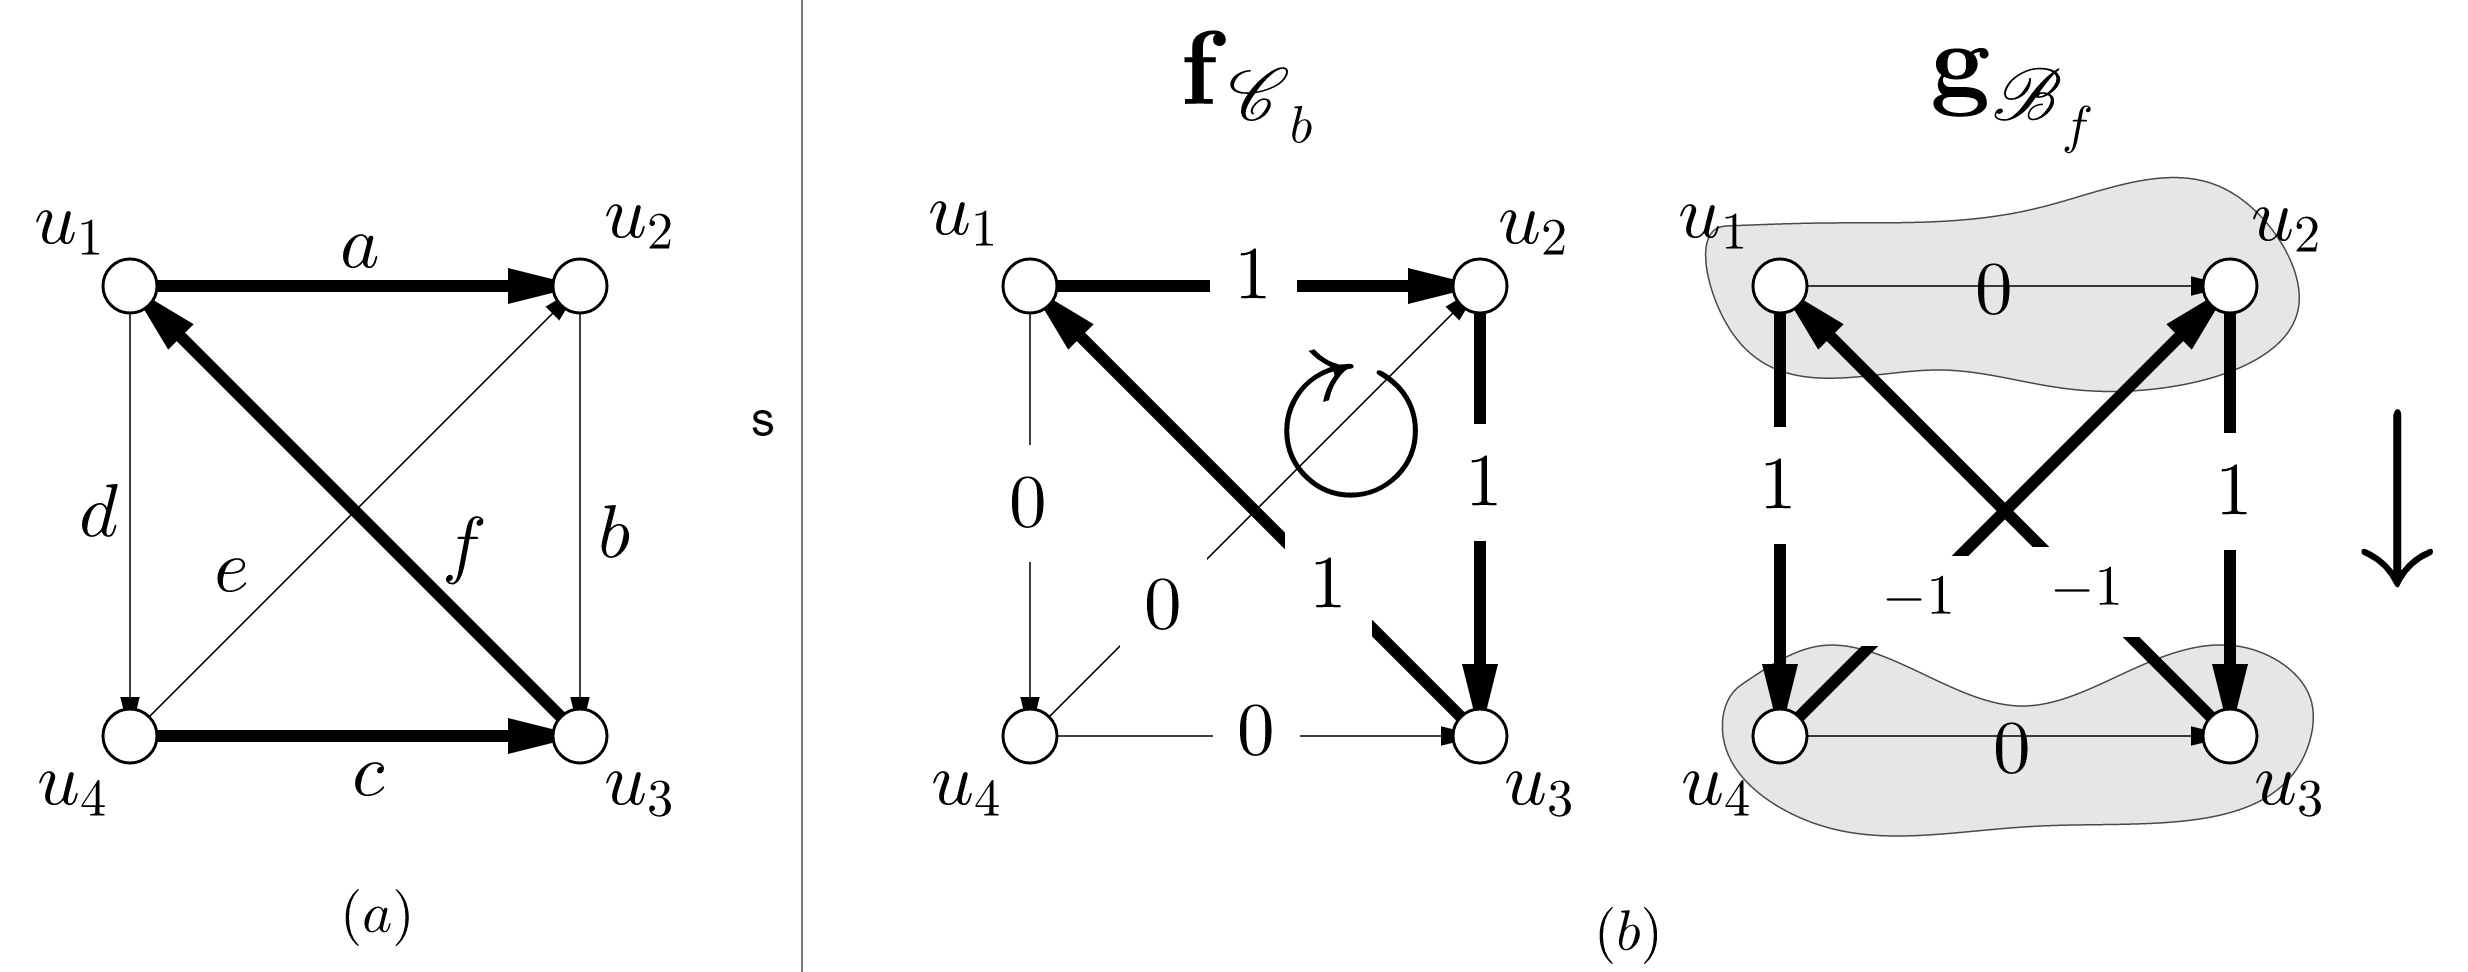
\includegraphics[scale=0.2]{img/imgchapter3/tensionescirculacionesfundamentales.jpg}
    \caption{}
    \label{fig:tensionescirculacionesfund}
\end{figure}
\hfill $\blacklozenge$
\end{ejem}
